\documentclass[titlepage]{article}
\usepackage[spanish]{babel}

% Set page size and margins
% Replace `letterpaper' with `a4paper' for UK/EU standard size
\usepackage[a4paper,top=2cm,bottom=2cm,left=3cm,right=3cm,marginparwidth=1.75cm]{geometry}

% Useful packages
\usepackage{amsmath}
\usepackage{graphicx}
\usepackage[colorlinks=true, citecolor=blue, linkcolor=black]{hyperref}

%%TABLES
\usepackage{multirow}
\usepackage{array} % required for text wrapping in tables

%%ÍNDICE
\usepackage{titlesec}
\usepackage{blindtext}

%%PSEUCODE
\usepackage[spanish, linesnumbered,ruled,vlined]{algorithm2e}

%%%CODE
\usepackage{listings}

%%BIBLIOGRAFIA
\usepackage{apacite}
\bibliographystyle{apacite}

%%INTERLINEADO DOBLE
\renewcommand{\baselinestretch}{2}

%%INTERLINEADO EN BLOQUES CONCRETOS
\usepackage{setspace}

%%FOOTNOTES
\usepackage[para]{footmisc}
\setlength{\skip\footins}{1cm}
\renewcommand{\footnotesize}{\scriptsize}

%%%%%TACHADO
\usepackage[normalem]{ulem}

%%IN-LINE CODE
\usepackage{listings}
\usepackage{color}
\definecolor{dkgreen}{rgb}{0,0.6,0}
\definecolor{gray}{rgb}{0.5,0.5,0.5}
\definecolor{mauve}{rgb}{0.58,0,0.82}

\lstset{frame=tb,
  language=Java,
  aboveskip=3mm,
  belowskip=3mm,
  showstringspaces=false,
  columns=flexible,
  basicstyle={\small\ttfamily},
  numbers=none,
  numberstyle=\tiny\color{gray},
  keywordstyle=\color{blue},
  commentstyle=\color{dkgreen},
  stringstyle=\color{mauve},
  breaklines=true,
  breakatwhitespace=true,
  tabsize=3
}

%%INFORMACIÓN
\title{¿En qué medida las técnicas de concurrencia optimizan el algoritmo de ordenación Merge Sort?}
\author{Gabriel Ruiz Díaz}
\date{}

%%% UNICODE
\usepackage[utf8]{inputenc}

%%%PGFPLOTS
\usepackage{pgfplots}
\pgfplotsset{compat=1.18}
%%%%CAPTION
\usepackage{caption}

%%%%%FIGURAS ADAPTADAS
\usepackage{wrapfig}

\begin{document}
%%%%PORTADA%%%%%%%%%%%%%%%%%
\begin{titlepage}
\centering
{\hfill}
\vspace{3cm}

{\Huge El algoritmo de ordenación por mezcla\par}
\vspace{2cm}
{\LARGE ¿En qué medida las técnicas de concurrencia optimizan el algoritmo de ordenación \textit{Merge Sort}? \par}
\vspace{1cm}
{\scshape\large Monografia de Informática NS \par}
\vspace{8cm}


{\Large Cómputo de palabras: xxxx \par}
{\Large Código del alumno: lqv708 \par}
\end{titlepage}

\newpage
\tableofcontents

\newpage
%%%%%%%%%%%%%%%INTRODUCIÓN%%%%%%%%%%%%%%%%%%%%%%
%%%%%%%%%%%%%%%%%%%%%%%%%%%%%%%%%%%%%%%%%%%%%%%%
\section{Introducción}
La finalidad de esta investigación evaluar holísticamente cuatro implementaciones del algoritmo de ordenación Merge Sort en términos de complejidad temporal y espacial, en el peor caso; tiempos de ejecución y memoria usados; y, la naturaleza específica de cada implementación. Concretamente, se comparan el Merge Sort Iterativo Serial (MSIS), el Merge Sort Recursivo Serial (MSRS), el Merge Sort Recursivo Paralelo (MSRP), y el Merge Sort Iterativo Paralelo (MSIP).


\subsection{Algoritmos de ordenación}
En el día a día usamos estructuras de datos ordenadas, como la lista de contactos del teléfono, en los almacenes para la gestión de inventario, en los resultados de una búsqueda en internet, etc. El proceso de colocar los datos en un cierto orden se llama ordenación.\footnote{\cite{knuth-1997}} La ordenación es una operación común en los sistemas informáticos y ha sido ampliamente estudiada.\footnote{\cite{McMillan-2007}} Aun así, no existe un algoritmo de ordenación perfecto. Actualmente, se siguen desarrollando, y además estos relacionan una gran variedad de conceptos de informática. Por ende, este estudio resulta relevante. En esta investigación, se aplican los paradigmas de la concurrencia, el paralelismo, la ejecución serial, la iteración y la recursión al algoritmo \textit{Merge Sort}.

\subsection{Merge Sort}
El ordenamiento por mezcla (\textit{Merge Sort}) es un algoritmo de ordenación inspirado en la técnica divide y vencerás (\textit{divide-and-conquer}). Es capaz de ordenar un conjunto de datos a través de los siguientes pasos: 
\begin{spacing}{1}
\begin{enumerate}
    \item dividir la colección en dos mitades,
    \item dividir las sub-colecciones en más mitades hasta que contengan cero o un elemento,
    \item ordenar cada sub-colección,
    \item unir (\textit{merge}) todas las sub-colecciones de forma ordenada, y, finalmente
    \item la colección queda ordenada.\footnote{\cite{skiena-2008}}
\end{enumerate}
\end{spacing}

\begin{figure}
    \centering
    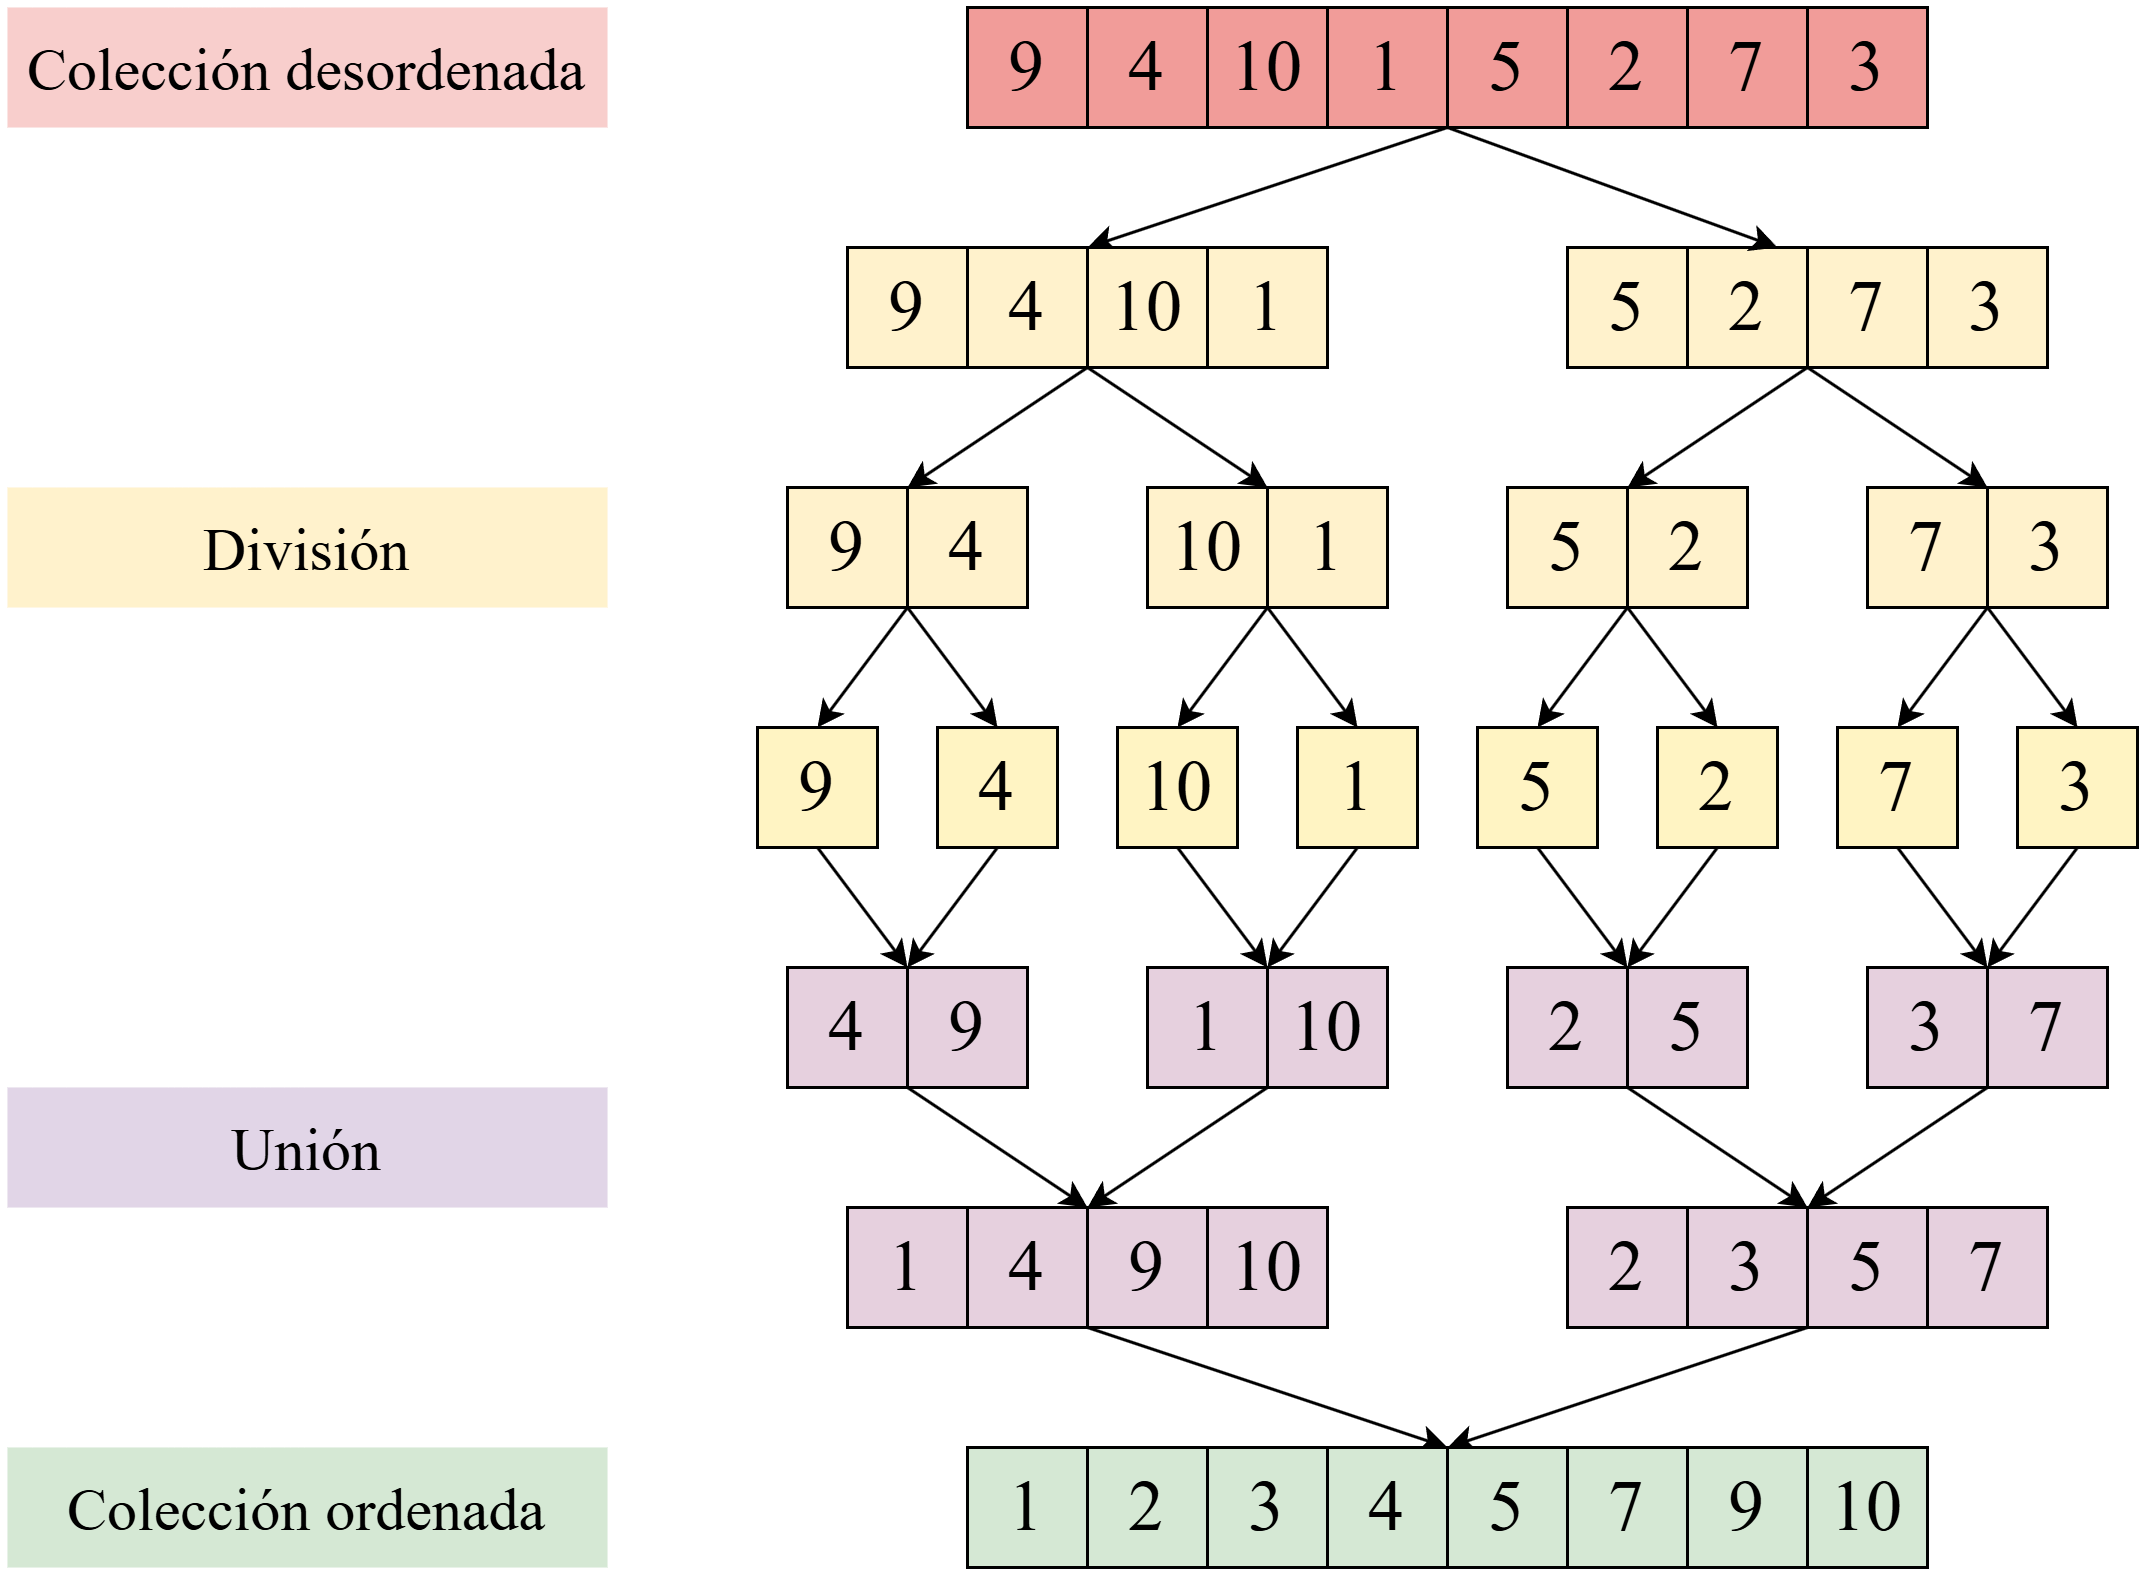
\includegraphics[width=0.75\linewidth]{Diagrames/arbolMS.png}
    \caption{Diagrama de árbol de \textit{Merge Sort}}
    \label{fig:arbolMS}
\end{figure}


\subsection{Concurrencia}
La concurrencia se refiere a la habilidad de un sistema para ejecutar múltiples tareas al mismo tiempo. \footnote{\cite{magee-2006}}.

\subsection{Ejecución serial y paralela}
Un \textbf{programa informático} es un conjunto de instrucciones que un sistema informático ejecuta. A su vez, un programa se divide en partes más pequeñas e independientes que llamamos tareas. Cuando las tareas se ejecutan una tras otra durante períodos de tiempo no superpuestos, hablamos de \textbf{ejecución serial}. A veces, la ejecución de una tarea depende del resultado de la tarea anterior. En dicho caso, la tarea bloquea a la siguiente. Esto es la \textbf{computación secuencial}. En contraposición, la \textbf{ejecución paralela }consiste en ejecutar varias tareas simultáneamente. Sin embargo, el paralelismo real solo es posible si el sistema consta de más de una unidad de procesamiento y si las tareas del algoritmo son independientes. \footnote{\cite{bobrov-2023}}

La idea es recorrer las dos partes izquierda y derecha del árbol del \textit{Merge Sort} (Figura \ref{fig:arbolMS}) paralelamente para aumentar la eficiencia del algoritmo.

\begin{figure}[htp]
    \centering
    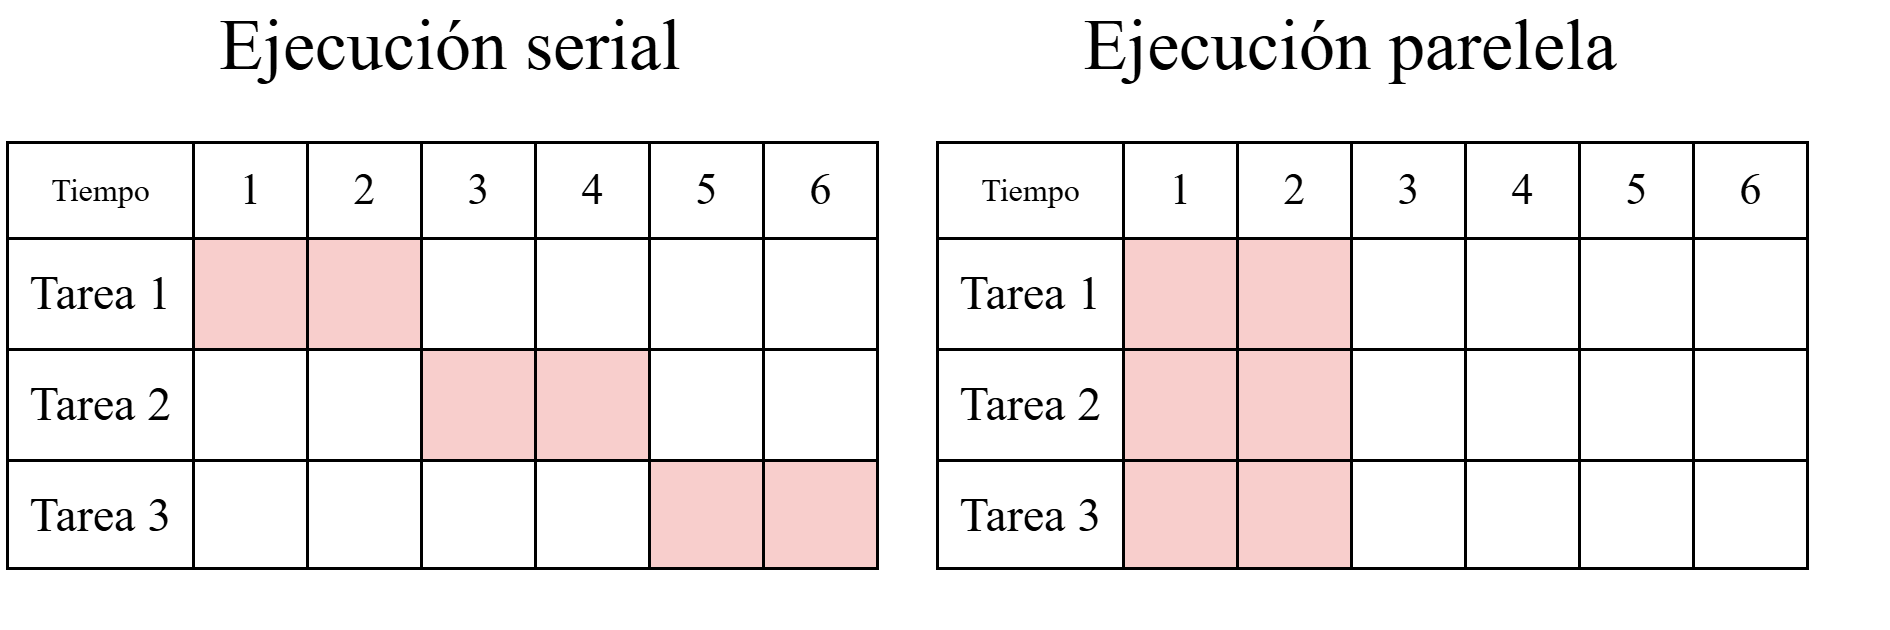
\includegraphics[width=0.75\linewidth]{Diagrames/serialVsParallel.png}
    \caption{Comparación de los diagramas de Gantt (//Nota: Probablemente cambiar por dos árboles mostrando la secuencia de instrucciones)}
    \label{fig:serialVsParallel}
\end{figure}

\subsection{Iteración y recursividad}
El paradigma de la \textbf{programación estructurada} considera que todo programa informático está formado por las estructuras de control de Secuencia, Selección y Repetición.\footnote{\cite{extended-learning-institute-no-date}} La recursión es una estructura de repetición.\footnote{\cite{wellesley-college-2000}} Si un programa incorpora una estructura recursiva, quiere decir que hay una función que se llama a sí misma. \footnote{\cite{bhargava-2016}} Toda función recursiva contiene caso recursivo, estructura condicional que llama a la propia función, y un caso base,  que retorna un valor constante o finaliza la función.

\textbf{[\\Nota: añadir gráfico para mostrar la recursión??]}

\subsection{Complejidad}
Esta investigación evalúa la aplicación de todos estos conceptos al algoritmo de ordenación por mezcla. La eficiencia de un algoritmo de ordenación usualmente se cuantifica en términos de complejidad temporal y espacial. La complejidad temporal es una medida de la variación del tiempo de ejecución de un algoritmo a medida que el tamaño de la entrada crece. El tiempo de ejecución se ve afectado por variables como el soporte físico y lógico (CPU, RAM, lenguaje de programación, SO...)\footnote{\cite{Heineman2008-mw}}Es por ello, que se estudia el comportamiento asintótico de la complejidad, es decir, cuando el tamaño de la entrada $n$ tiende al infinito. Lo hace mediante las funciones del: peor caso posible \(O(n)\), el caso promedio \(\theta(n)\), y el mejor caso posible \(\Omega(n)\). \footnotemark[8] De ahí la notación \textit{Big-O}, que permite comparar algoritmos a través de distintas plataformas y predecir el tiempo de ejecución de un algoritmo.

La complejidad temporal se mide usualmente mediante la función del peor caso posible por varios motivos: es más sencillo de analizar al no ser necesario conocer la distribución de datos de entrada, garantiza el buen funcionamiento del programa en el que se incorpore en caso de situaciones desfavorables... Caracterizar un algoritmo mediante su complejidad \(O(n)\) es una abstracción, ya que se fundamenta en el modelo de Máquina de Acceso Aleatorio, que considera que las \textit{operaciones básicas}, como las aritméticas, lógicas o los accesos a la memoria, duran una sola unidad de tiempo. Asimismo, se considera que cada línea de código es una \textit{instrucción básica} que ejecuta un número constante de operaciones básicas. Los bucles (\lstinline{for}, \lstinline{for, while...} y llamadas a funciones se evalúan sumando sus instrucciones básicas.

La notación \textit{Big-O} proporciona un límite superior para el cual una función nunca lo sobrepasará. Esta notación estudia el orden de crecimiento de una función. Formalmente, se define como: dadas dos funciones \(f(n)\), \(g(n)\), entonces \(f(n) = O(g(n))\) siempre que existan las constantes \(c\) y \(n_0\) tal que \(f(n) \leq c\cdot g(n)\), para todo \(n \geq n_0\). Esto significa que para una función \(f(n)\) solo existirá un Big-O \(O(g(n))\) si todos los valores de su entrada \(n\) son inferiores al producto entre una constante \(c\) y una función \(g(n)\), que es el límite superior. De forma que, \(f(n)\) nunca crecerá más que \(g(n)\).

\begin{wrapfigure}{r}{0.4\textwidth}
\captionsetup{justification=centering}
\centering    
        \begin{tikzpicture}[scale=0.8]
            \begin{axis}[
                xlabel={Entrada $n$},
                ylabel={Tiempo de ejecución $y$}, 
                xmin=0, xmax=20, 
                ymin=0, ymax=100, 
                xtick={0,5,10,15,20,7},
                legend pos=north west, 
                grid=major,
                grid style={dashed, gray!30} 
            ] 
            \addplot[ 
                domain=0:20, 
                samples=20, 
                color=blue,thick 
            ]{4*x + 7}; 
            \addlegendentry{$f(n) = 4n + 7$} 
            \addplot[ 
                domain=0:20, 
                samples=20, 
                color=orange, thick 
            ]{5*x}; 
            \addplot[ 
                color=black, dashed, thick 
            ] coordinates{(7,0) (7,35)};
            
            \addlegendentry{$g(n) = 5n$} 
            \end{axis}
        \end{tikzpicture}
    
    \caption{Ejemplo de \textit{Big-O}}
    \label{fig:bigO}
    
\end{wrapfigure}

Por ejemplo, se da un algoritmo que toma un tiempo de ejecución \(f(n) = 4n+7\) y queremos saber si se comporta de forma lineal. Esto es \(g(n)=n\) Entonces para que \(f(n) = O(g(n))\) hay que encontrar un valor de \(c\) para el que se cumpla que \(4n+7 \leq c\cdot n\). Con \(c=5\) la inecuación se cumple, por tanto: \(f(n) = O(g(n)) = O(n)\); y esto solo se cumple para \(n \geq n_0\), en este caso \(n\geq 7\) porque: \(4n+7 \leq 5n \space \rightarrow 7 \leq 5n - 4n   \rightarrow 7 \leq n\). De forma que el \textit{Big-O} de \(4n+7\) es \(O(n)\) para cualquier entrada mayor que \(7\).



\section{Implementaciones}

\subsection{Merge Sort Recursivo Serial (MSRS)}
El algoritmo de ordenación por mezcla clásico se basa en el paradigma <<divide y vencerás>>. Es decir, primero se divide un problema en otros subproblemas, se solucionan los subproblemas, y, se combinan para llegar a la solución
final.\footnote{\cite{Sedgewick2003-cd}}

\begin{figure}[hbtp]
    \begin{lstlisting}[language=java, frame=single, numbers=left]
        public static void sort(int[] A, int length) {
            if (length <=1) return;
    
            int mid = length / 2;
            int[] L = new int[mid];
            int[] R = new int[length - mid];
    
            for (int i = 0; i < mid; i++)   L[i] = A[i];
            for (int i = mid; i < length; i++)  R[i - mid] = A[i];
    
            sort(L, mid);
            sort(R, length - mid);
    
            merge(A, L, R, mid, length - mid);
        }
    \end{lstlisting}
    \caption{Función \lstinline{sort()} del Merge Sort Recursivo Serial}
    \label{fig:MSRS_sort()}
\end{figure}

Como se observa en la Figura \ref{fig:MSRS_sort()} el algoritmo a estudiar consta de una función \lstinline{sort()} que toma una colección \lstinline{A} y su longitud \lstinline{length}. Después calcula el pivote \lstinline{mid} desde donde dividir la colección original \lstinline{A}, instancia dos colecciones locales, \lstinline{L} y \lstinline{R}, y copia los elementos de \textit{A} a cada mitad. Estas mitades se ordenan independientemente a través de las llamadas recursivas de las líneas 11 y 12 a \lstinline{sort()}. 

\begin{figure}[hbtp]
    \begin{lstlisting}[language=java, frame=single, numbers=left]
        public static void merge(int[] A, int[] L, int[] R, int left, int right) {
            int i = 0, j = 0, k = 0;
    
            while (i < left && j < right)   A[k++] = (L[i] <= R[j])? L[i++] : R[j++];
    
            while (i < left)    A[k++] = L[i++];
            while (j < right)   A[k++] = R[j++];
        }
    \end{lstlisting}
    \caption{Función \lstinline{merge()} del Merge Sort Recursivo Serial}
    \label{fig:MSRS_merge()}
\end{figure}

Finalmente, se unen las mitades mediante la función \lstinline{merge()} de la Figura \ref{fig:MSRS_merge()} que toma la colección original \lstinline{A}, y las sub-colecciones \lstinline{L} y \lstinline{R}, además de sus respectivas longitudes \lstinline{left}, \lstinline{right}. Para controlar el recorrido de las tres colecciones se emplean tres índices: \lstinline{i} para \lstinline{L}, \lstinline{j} para \lstinline{R} y \lstinline{k} para \lstinline{A}. Un primer bucle coloca en \lstinline{A[k]} el elemento más pequeño entre \lstinline{L[i]} y \lstinline{L[j]} sucesivamente. Los dos bucles posteriores colocan en \lstinline{A[k]} los elementos no colocados en el bucle anterior. Por último, en caso de que una mitad se haya recorrido por completo, la restante se copia en \lstinline{A}.

\subsubsection{Complejidad}
La complejidad temporal del algoritmo será la suma de las complejidades de cada línea. Según el modelo MAN, la comprobación del caso base (línea 2, Figura \ref{fig:MSRS_sort()}) y el cálculo del pivote \lstinline{mid} toman tiempo constante \(O(1)\) al ser operaciones básicas. La inicialización de \lstinline{L} y \lstinline{R} toma tiempo \(O(n)\) porque en Java la creación de un arreglo implica la asignación de espacio en la memoria proporcional al tamaño de este, en este caso \lstinline{lenght = }\(n\). La copia de las sub-colecciones (bucles de las líneas 8-9) toman \(O(n)\) al su tiempo de ejecución depender de \(n\). Por último, \lstinline{merge} (Figura \ref{fig:MSRS_merge()}) toma \(O(n)\) porque en el peor caso se realizaran \lstinline{left} \(+\) \lstinline{right} \(=\) \lstinline{lenght} comparaciones \lstinline{L[i]<=R[j]}, que es lo mismo que \(n\). Por tanto, el tiempo de ejecución respecto la entrada por ahora es \(f(n) = 2O(1) + 2O(n) + 2O(n)+ O(n)\), que es igual a \(O(n)\) ya que según la notación \textit{Big-O} se ignoran los términos de menor orden y los factores constantes, puesto que estos no afectan significativamente al crecimiento cuando \(n\) tiende a un número grande.

\begin{figure}[hbtp]
    \centering
    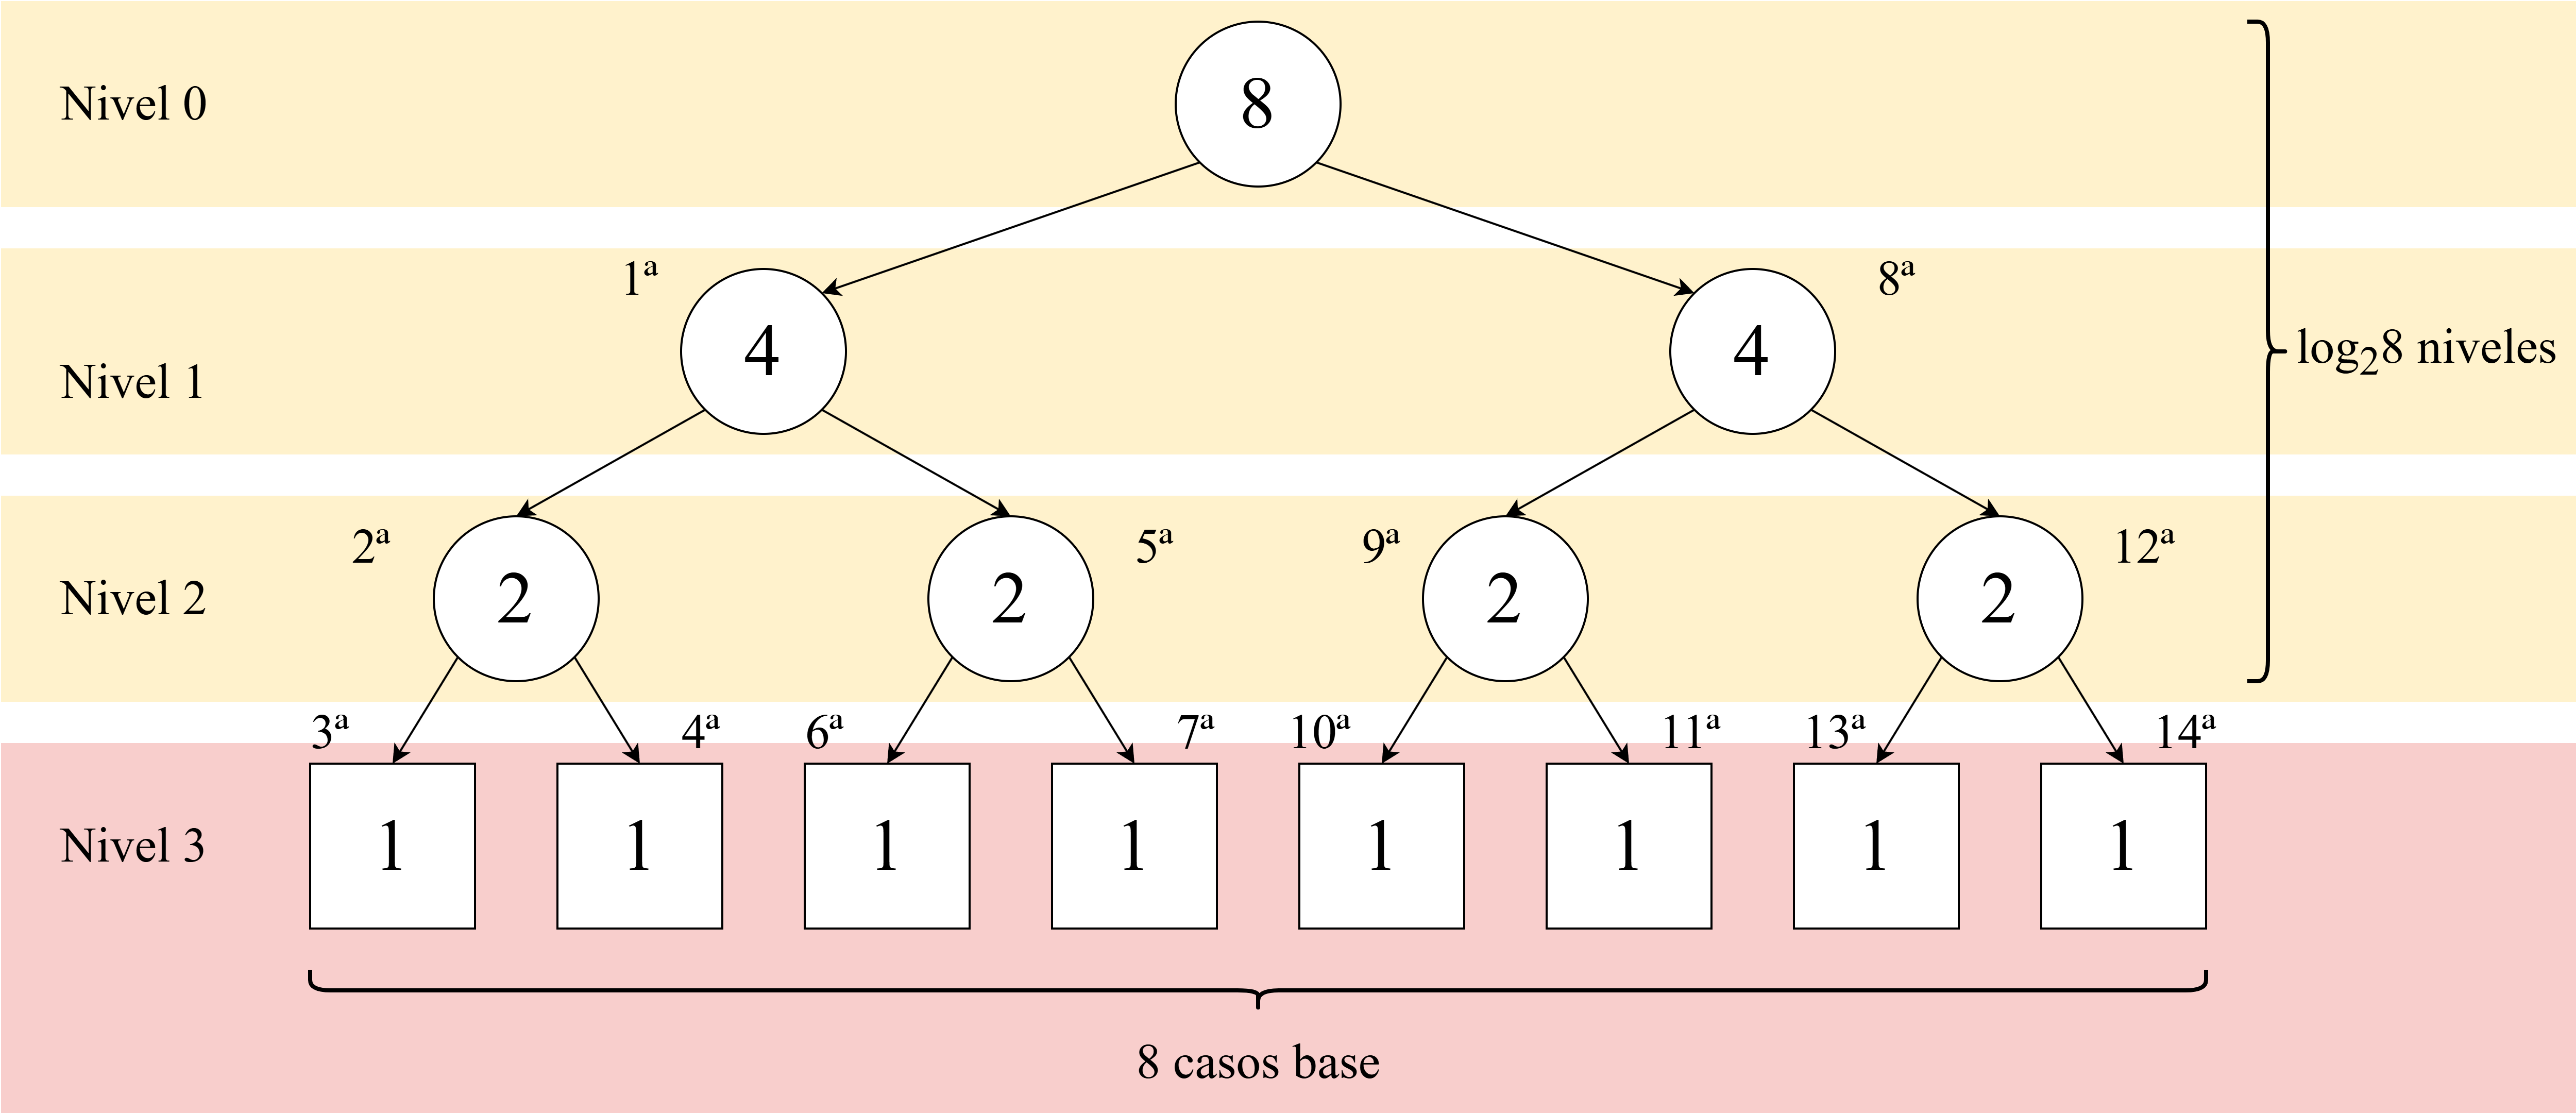
\includegraphics[width=0.8\linewidth]{Diagrames/arbolBinarioMSRSn8.png}
    \caption{Árbol binario para \(n=8\)}
    \label{fig:arbol-MSRS-N=8}
\end{figure}

Lo anterior corresponde a una llamada a \lstinline{sort()}, pero esta función es recursiva, por tanto, hay que determinar cuantas veces se llama a \lstinline{sort()} en función del tamaño de la entrada \(n\). Estos se facilita si rastreamos las llamadas a \lstinline{sort()}, por ejemplo mediante un árbol binario como el de la Figura \ref{fig:arbol-MSRS-N=8} donde cada nodo representa la longitud de la entrada \lstinline{lenght}. Se observa que para 8 llamadas hay tres niveles en el árbol, la relación entre 8 y 3 es que \(log_{2}{3} = 3\) ya que \(8=2^3\). Por extensión, para un \(n\) tamaño de entrada hay \(\log_{2}{n}\) niveles. Esto se cumple siempre que \(n\) sea múltiplo de 2, lo que da lugar a un árbol simétrico como el de Figura \ref{fig:simetriaMSRS}, en caso contrario es asimétrico y hay llamadas extras. El trabajo realizado en cada nivel \(i\) es \(2^i\cdot n \cdot \frac{n}{2^i} = n\) como se observa en la Figura \ref{fig:entradaMSRS} donde \(n\) es el tamaño de entrada original. Finalmente, el trabajo \(f(n)\) de una llamada a \lstinline{sort()} es la suma del trabajo en cada nivel, menos el del último nivel porque los casos bases requieren \(O(1)\) al realizarse un \lstinline{return}. Esto es:
\[f(n) = \sum_{i=0}^{\log_{2}{n} -1} {n} = n\sum_{i=0}^{\log_{2}{n} -1} {1} = n\cdot\log_{2}{n}\]
A continuación se aplica la definición de la notación \textit{Big-0}, donde \(f(n)=n\log_{2}{n}\) y \(g(n)=n\log{n}\). Existe un \(f(n)=O(n\log{n})\) siempre que: 
\[n\log_{2}{n} \leq c\cdot n\log{n}\]
Aislamos la constante \(c\):
\[n\log_{2}{n} \leq c\cdot n\log{n} \longrightarrow c \geq \frac{\log_{2}{n}} {\log_{10}{n}} \longrightarrow c \geq \frac{ \frac{\log_{10}{n}} {\log_{10}{2}} } {\log_{10}{n}} \longrightarrow c \geq \frac{1}{\log{2}} \]
Esto significa que la complejidad del MSRS se aleja de \(O(n\log_n)\) en un factor aproximado de \(3,32\%\) siempre que la entrada sea mayor que 1 y sea múltiplo de 2. Aun así, la literatura considera que el \textit{Merge Sort} tiene complejidad \(O(n\log{n})\) por razones prácticas. \footnote{\cite{Sedgewick2003-cd}}

\begin{figure}[h]
\centering 
\captionsetup{justification=centering, margin=10pt}
\begin{minipage}{0.5\textwidth} 
    \centering 
    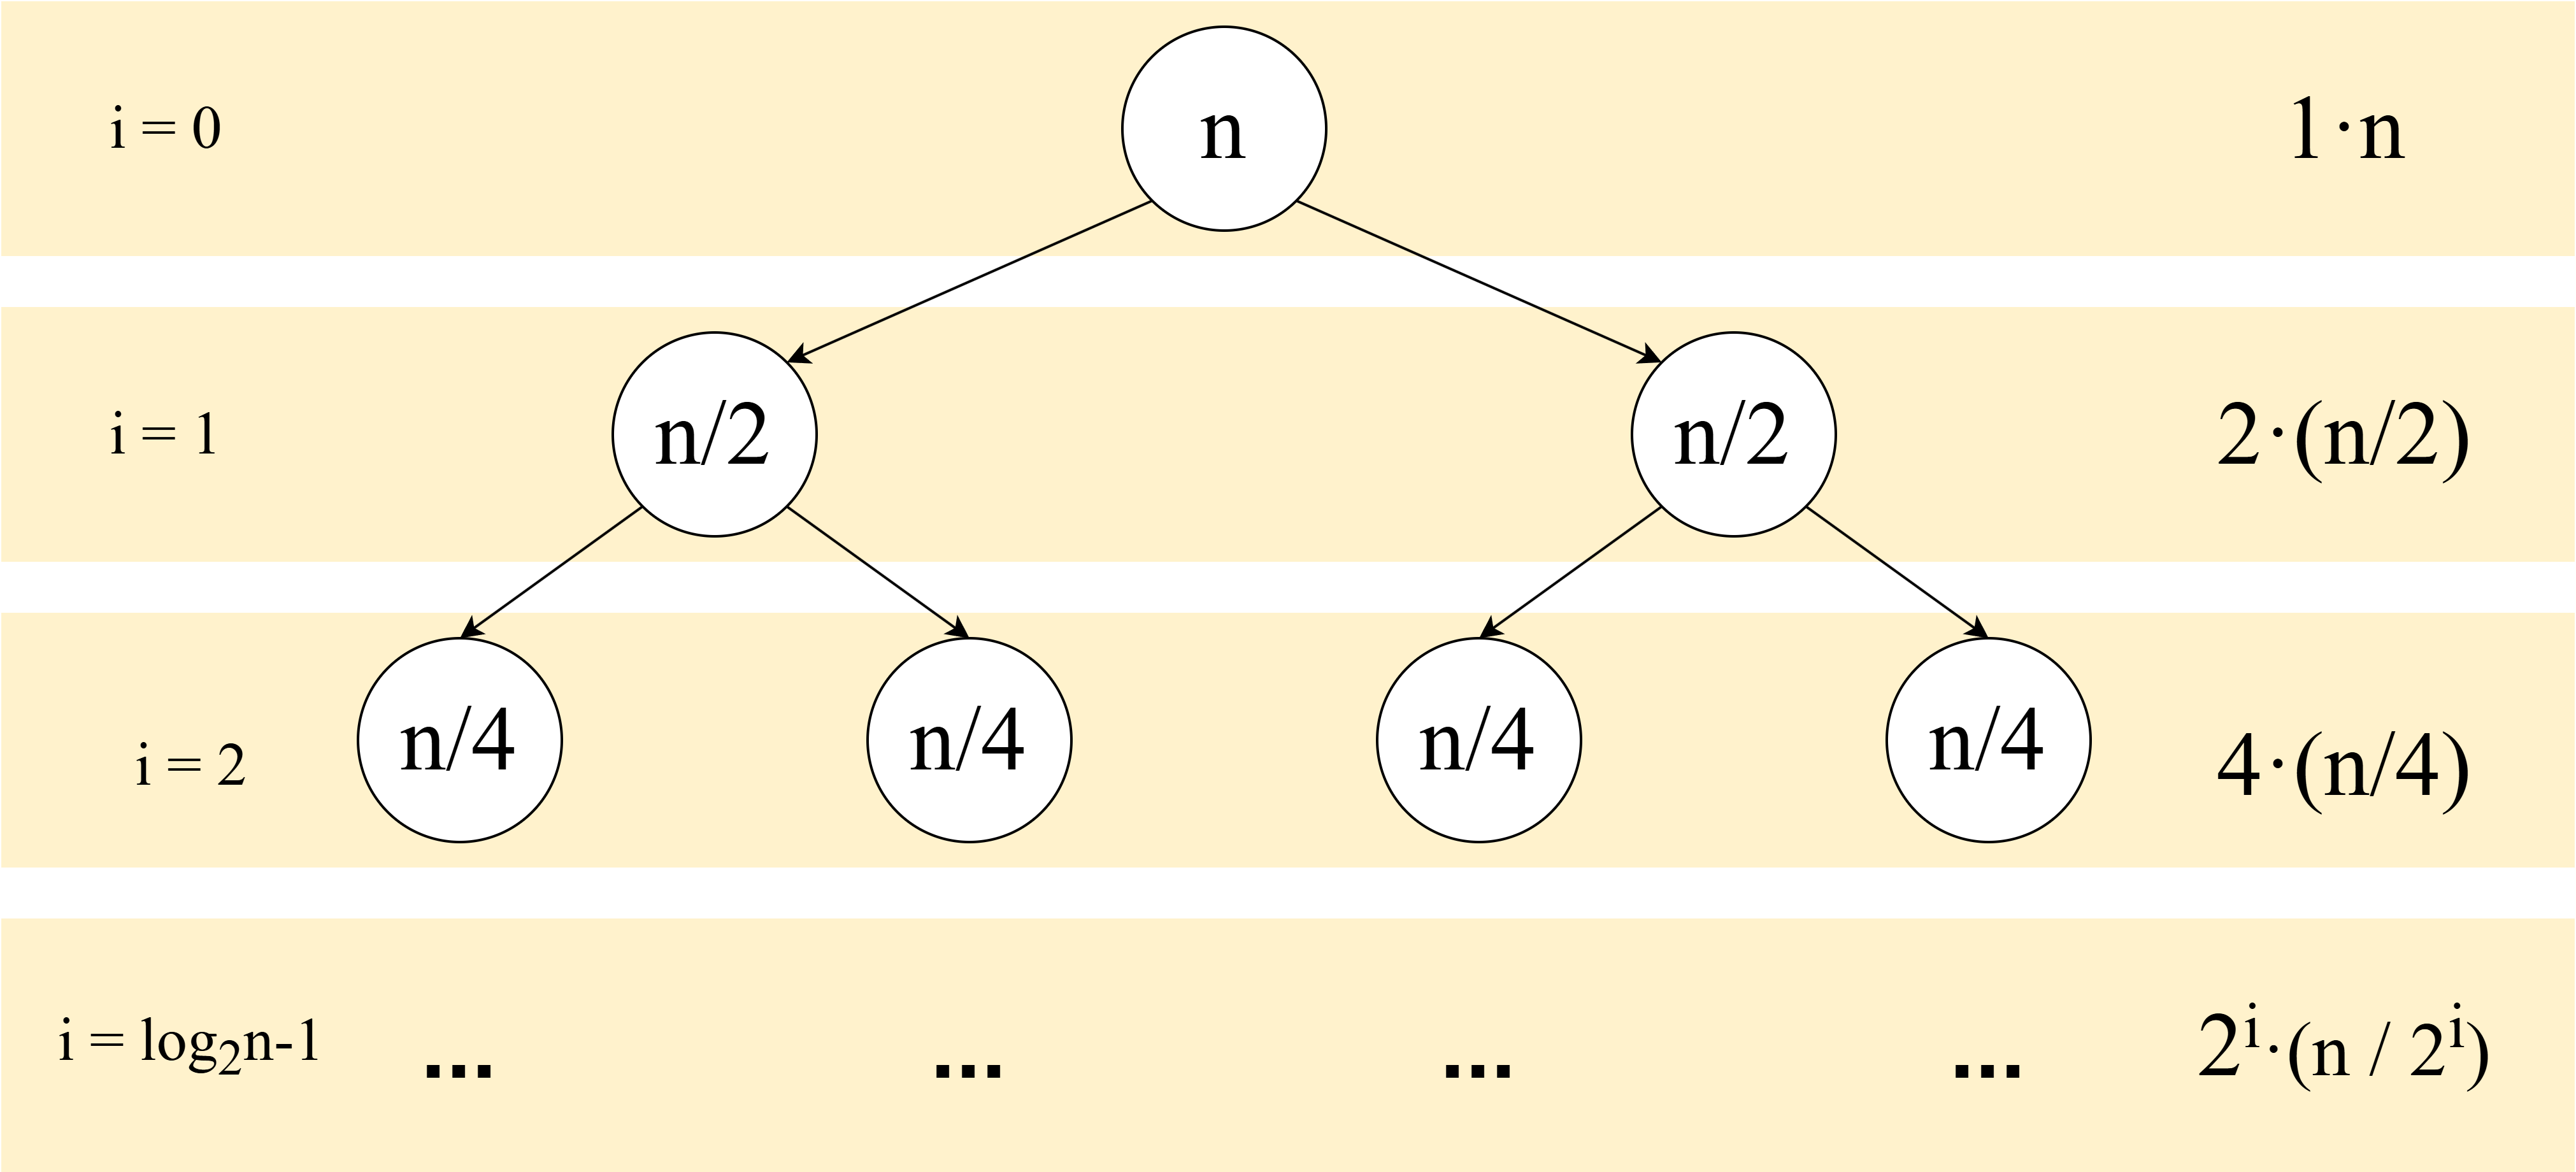
\includegraphics[width=0.95\linewidth]{Diagrames/arbolBinarioLenght.png} 
    \caption{Tamaño de la entrada a lo largo de las llamadas a \lstinline{sort()}} 
    \label{fig:entradaMSRS}
\end{minipage}\hfill 
\begin{minipage}{0.5\textwidth} 
    \centering 
    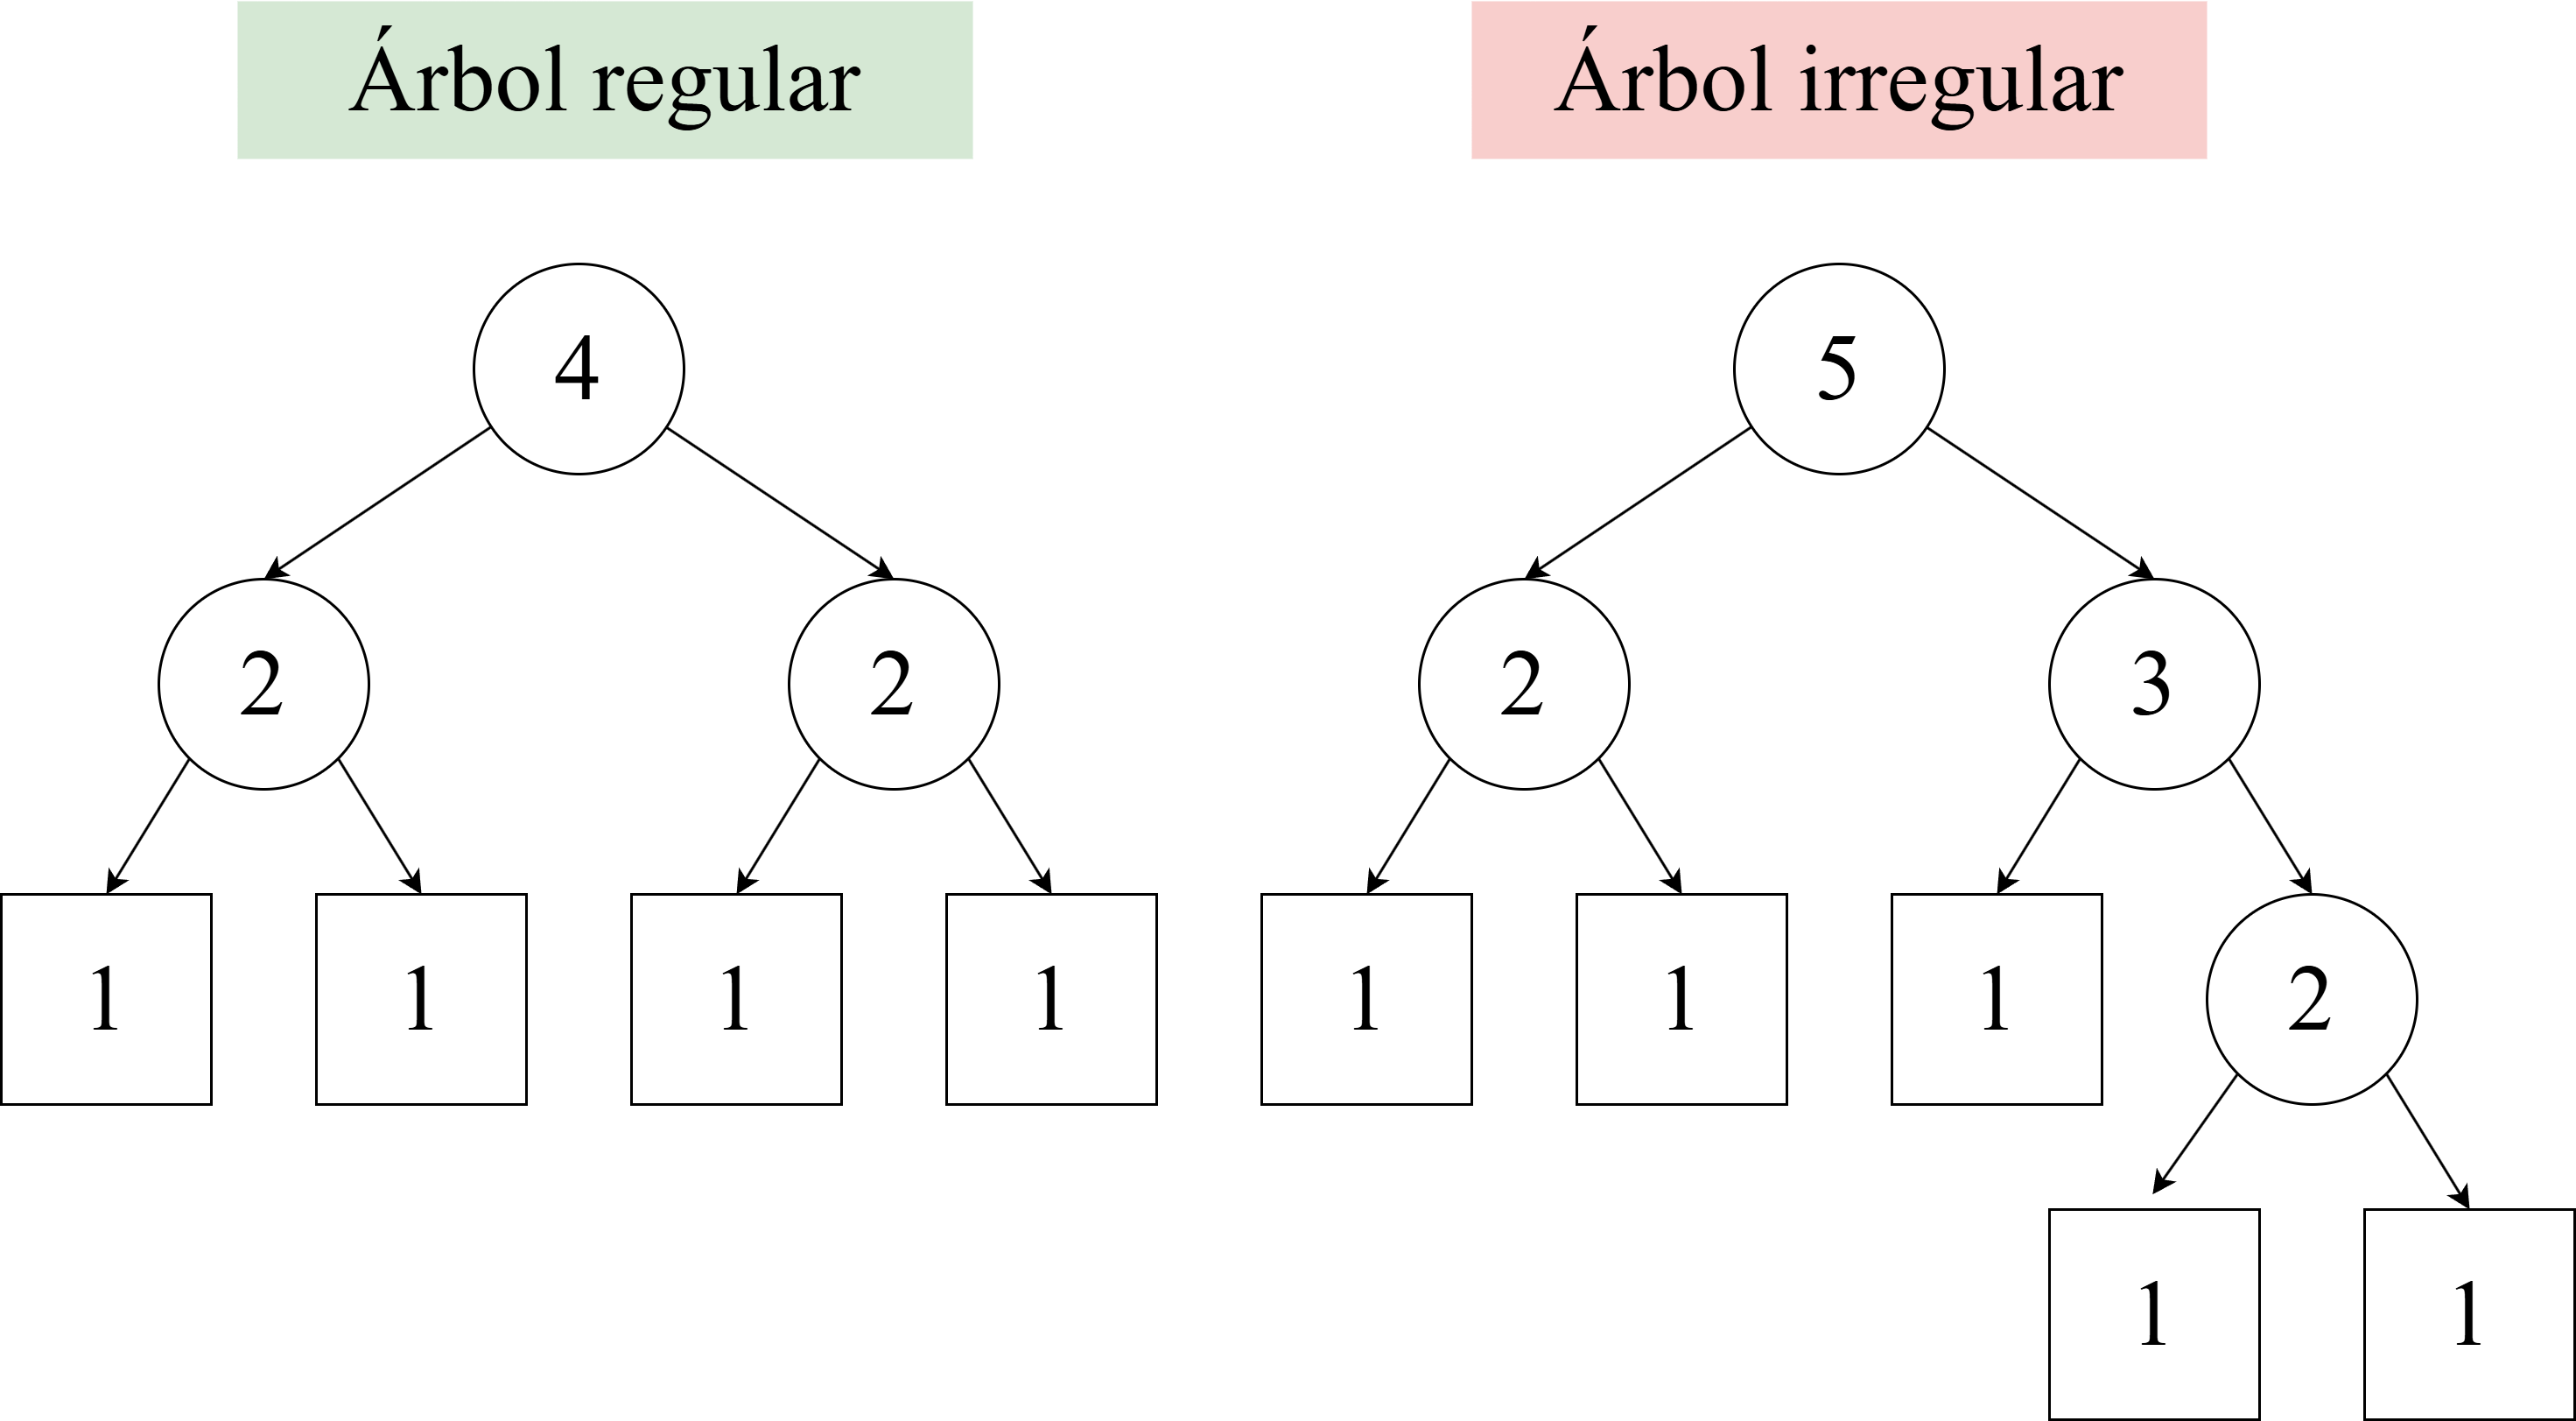
\includegraphics[width=0.95\linewidth]{Diagrames/arbolBinario_MSRS.png} 
    \caption{Árbol simétrico verus árbol asimétrico del MSRS} 
    \label{fig:simetriaMSRS}
\end{minipage} \end{figure}

\subsection{Merge Sort Iterativo Serial (MSIS)}

El MSIS es la versión análoga al clásico MSRS, en esta implementación (Figura \ref{fig:MSIS_sort()}) se divide la colección en partes más pequeñas, después las partes adyacentes se unen, y se aumenta el tamaño  de las partes. Estos tres pasos se repiten hasta que la parte tenga el tamaño de la colección original. El primer bucle determina el tamaño \lstinline{lenght} de las partes: \lstinline{size} \(=2, 4, 8..\). El segundo bucle determina el índice \lstinline{left} desde el cual comienza la parte \lstinline{arr[left]...arr[left+size-1]} que será unida a su adyacente \lstinline{arr[mid]...arr[right]} mediante \lstinline{merge()}. Este índice toma valores en intervalos de \lstinline{2*size}. En la Figura \ref{fig:ejecuciónMSIS} se presenta el proceso de ordenación de una colección: las casillas coloreadas representan las sucesivas iteraciones de \lstinline{left} del segundo bucle; las casillas azules corresponden a la respectiva parte izquierda de una iteración; y las verdes la parte derecha.

\begin{figure}[hbtp]
    \begin{lstlisting}[language=java, frame=single, numbers=left]
        public static void sort(int[] arr) {
            int n = arr.length;
            int[] aux = new int[n];
    
            for (int size = 1; size < n; size *= 2) {
                for (int left = 0; left < n - size; left += 2 * size) {
                    int mid = left + size - 1;
                    int right = Math.min(left + 2 * size - 1, n - 1);
                    merge(arr, aux, left, mid, right);
                }
            }
        }
    \end{lstlisting}
    \caption{Función \lstinline{sort()} del Merge Sort Iterativo Serial}
    \label{fig:MSIS_sort()}
\end{figure}

\begin{figure}
    \centering
    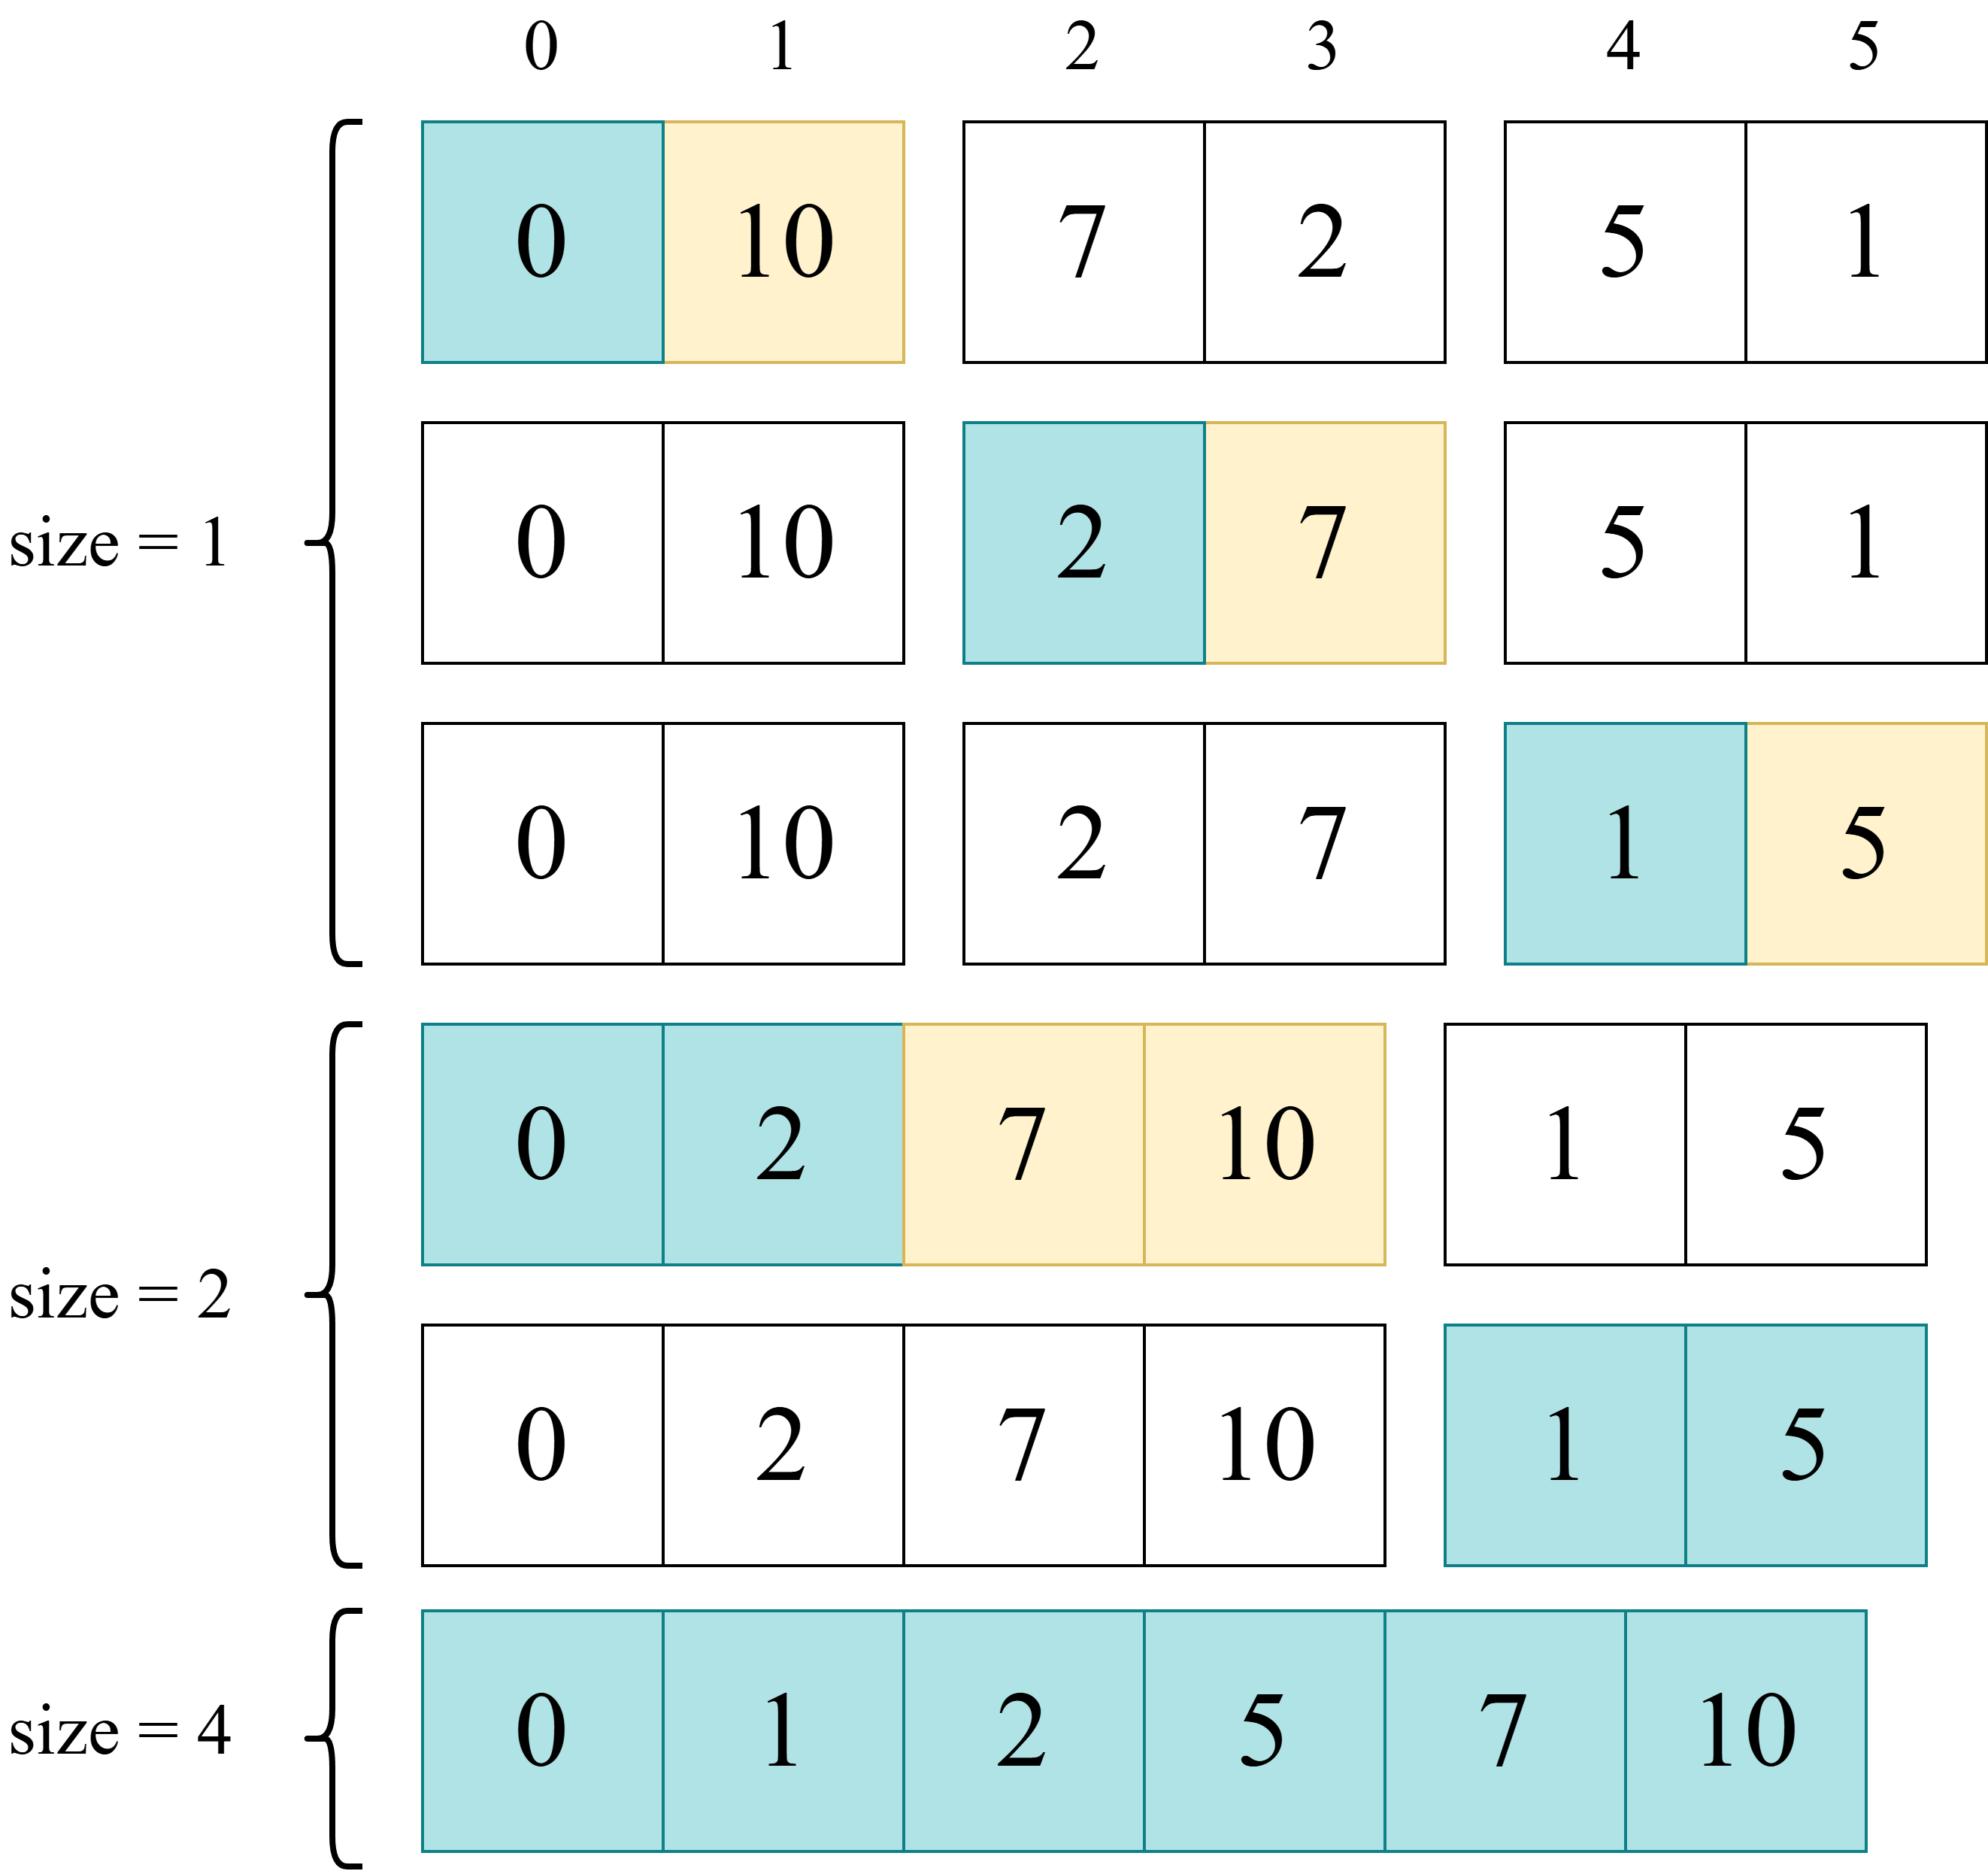
\includegraphics[width=0.5\linewidth]{Diagrames/ejecucionMSIS.png}
    \caption{Ejecución del Merge Sort Iterativo Serial}
    \label{fig:ejecuciónMSIS}
\end{figure}

Dado que las partes son de longitud variable, se ha modificado la función \lstinline{merge()} anterior para no depender de dos colecciones auxiliares, sino de una sola. En esta implementación \lstinline{arr[left]...arr[mid]} es una parte que se une a su adyacente \lstinline{arr[mid+1]...arr[right]}. Las dos partes y la colección original se recorren mediante los índices \lstinline{i}, \lstinline{j}, \lstinline{k} respectivamente.

\begin{figure}[hbtp]
    \begin{lstlisting}[language=java, frame=single, numbers=left]
        private static void merge(int[] arr, int[] aux, int left, int mid, int right) {
            for (int i = left; i <= right; i++) aux[i] = arr[i];
            int i = left, j = mid + 1, k = left; 
            
            while (i <= mid && j <= right) arr[k++] = (aux[i] <= aux[j])? 
            aux[i++] : aux[j++];
            while (i <= mid) arr[k++] = aux[i++];
        }    
    \end{lstlisting}
    \caption{Función \lstinline{merge()} del Merge Sort Iterativo Serial}
    \label{fig:MSIS_merge()}
\end{figure}

\subsubsection{Complejidad temporal}
Si se observa el árbol binario de la Figura \ref{fig:arbolMSIS}, el MSIS recorre el árbol desde la base de la recursión hasta la parte superior, ya que se realizan uniones entre partes de 1-1, 2-2- 4-4... Como en el MSRS, el árbol será simétrico solo si el tamaño de entrada en múltiplo de 2. Siguiendo el mismo método y tomando las mismas suposiciones que en el cálculo de la complejidad temporal del MSRS, la complejidad del MSRS es \(O(n \log{n})\) porque hay \(\log_2{n}-1\) llamadas a \lstinline{sort()} en las cuales se realiza un trabajo de \(O(n)\) en el peor caso.

\begin{figure}
    \centering
    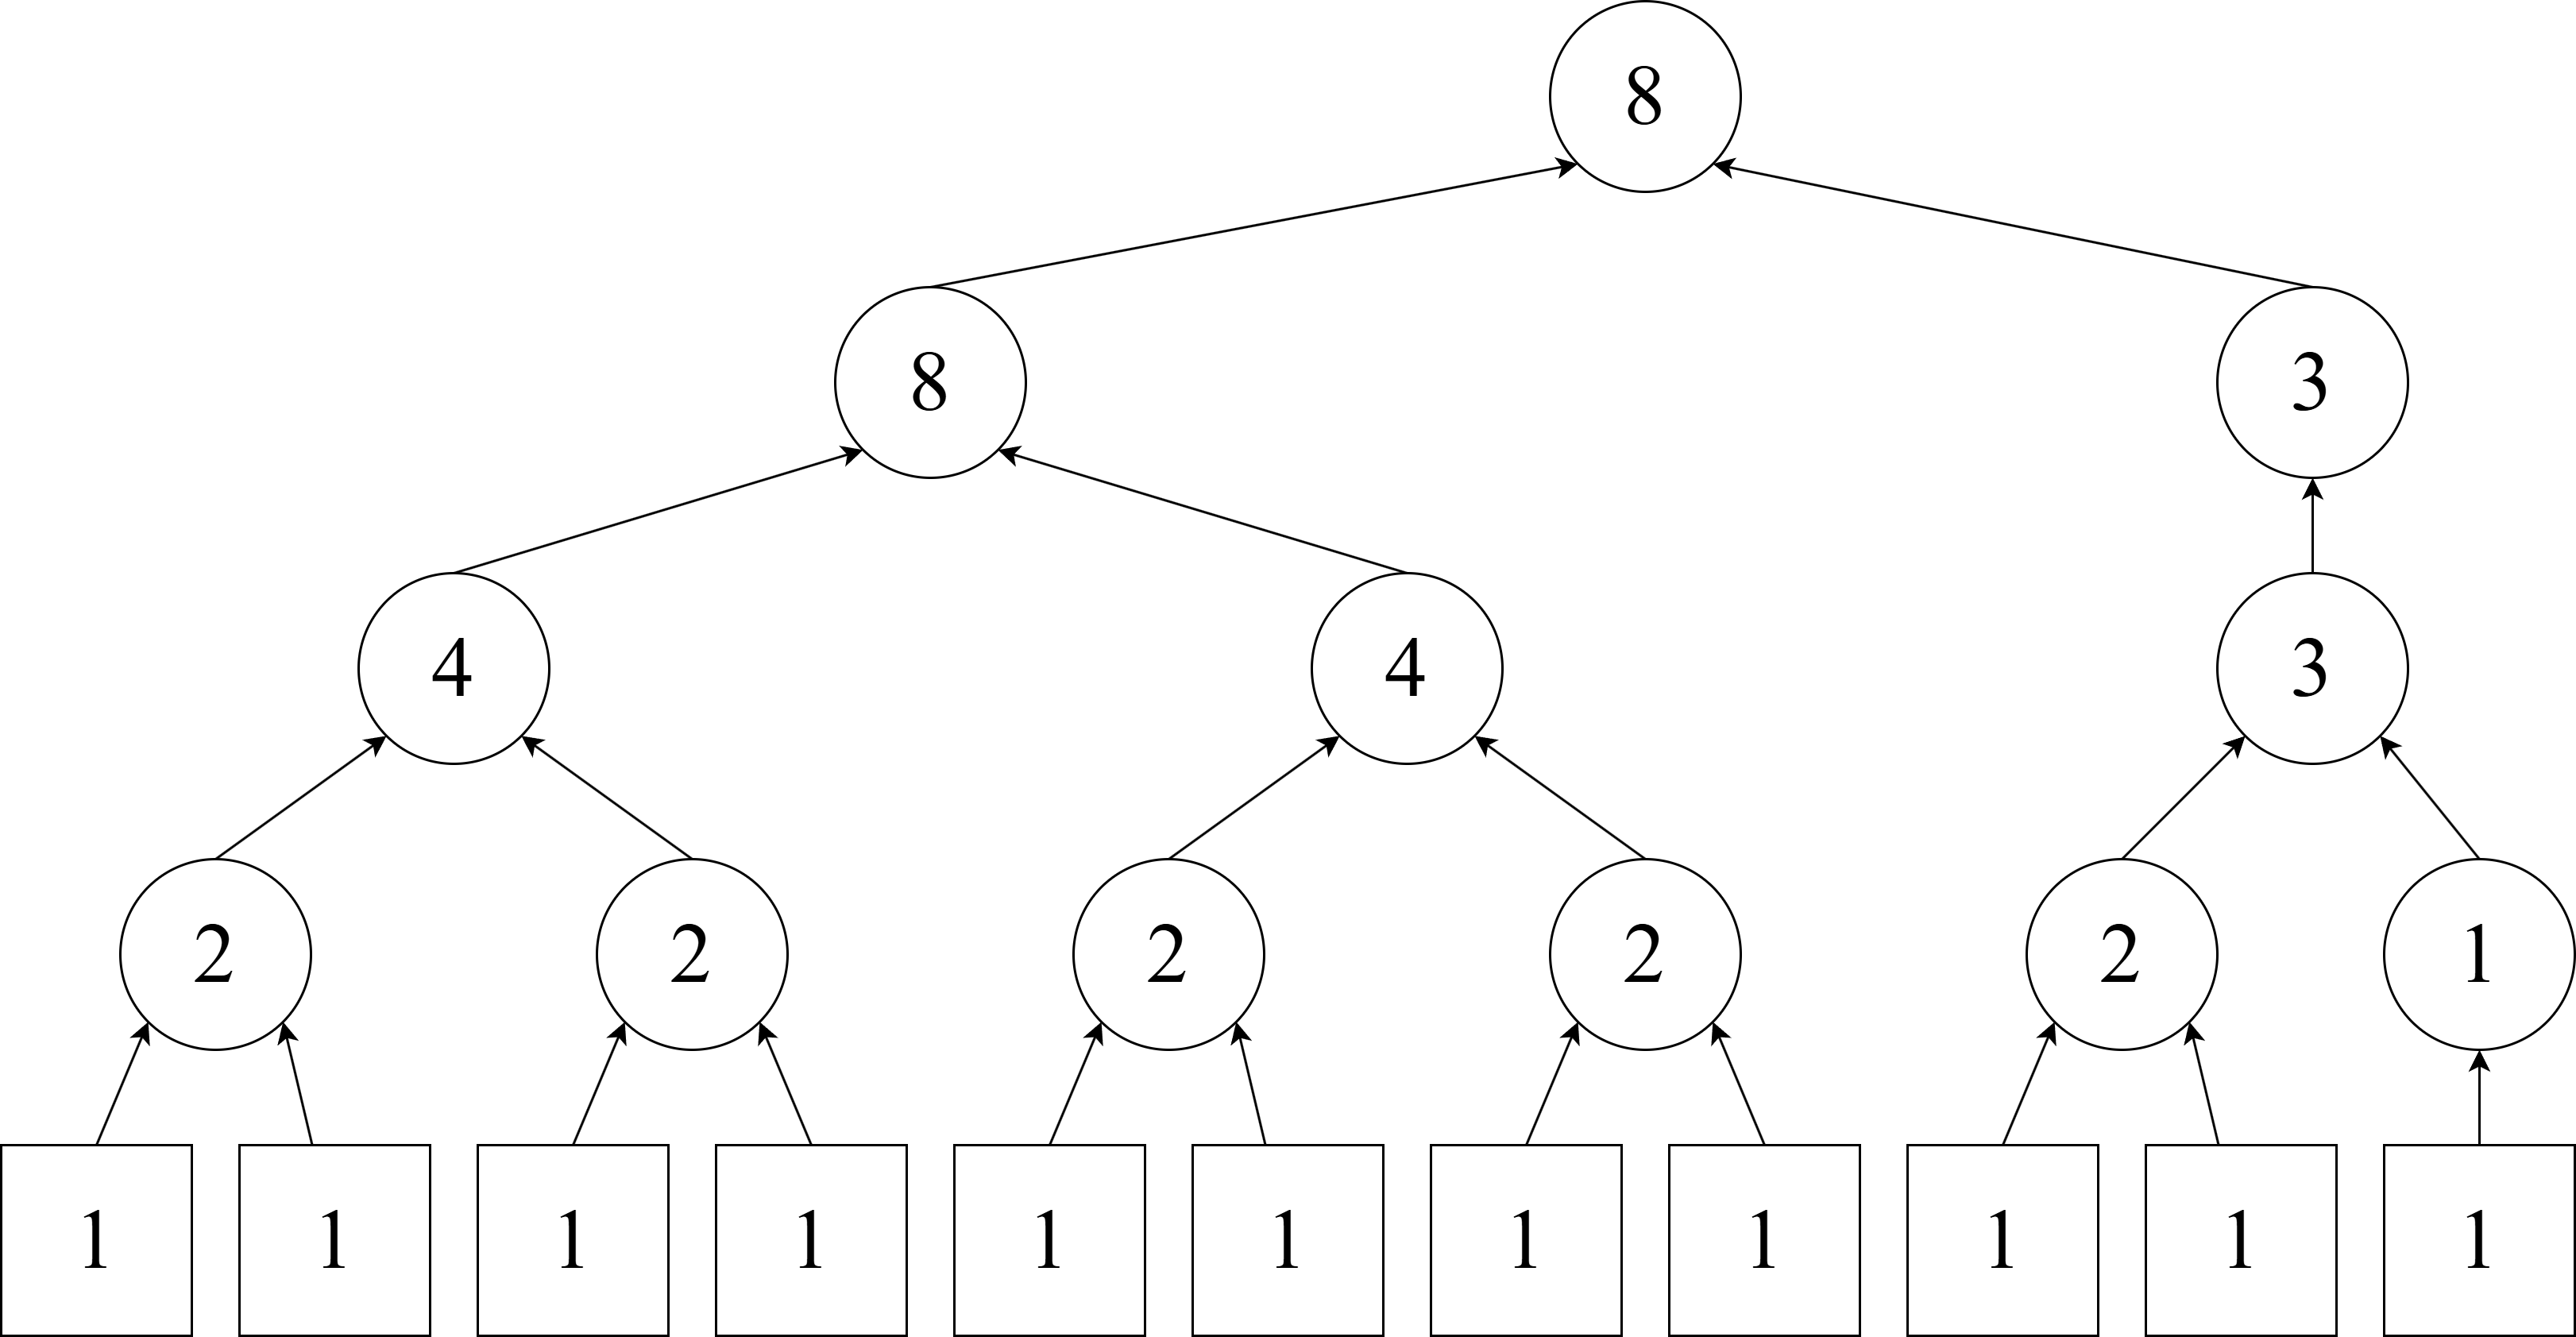
\includegraphics[width=0.8\linewidth]{Diagrames/arbolMSISirregular.png}
    \caption{Árbol binario del Merge Sort Iterativo Serial}
    \label{fig:arbolMSIS}
\end{figure}

\subsection{Merge Sort Recursivo Paralelo (MSRP)}
Un proceso es la ejecución de las instrucciones de un programa, después de que estas instrucciones se hayan movido desde la memoria secundaria (SSD por ejemplo) hasta la primaria (RAM). El sistema operativo en quien se encarga de crear los procesos y guarda en la memoria la información asociada al proceso: un identificador de proceso único (\textit{PID}); un espacio de direcciones de memoria, ya que un proceso lee y modifica datos guardados en la memoria; el estado del proceso; y, una lista de los archivos que el programa usa. En cambio, un hilo de ejecución es una secuencia de instrucciones que el planificador del sistema operativo puede manejar independientemente. \footnote{\cite{bobrov-2023}} Hasta se han mostrado programas que al ejecutarse toman la forma de un proceso con un solo hilo de ejecución. La idea es mejorar el rendimiento del \textit{Merge Sort} haciendo uso de más de un hilo de ejecución. 

La herramienta más apropiada que proporciona Java para esta tarea es la clase \lstinline{ForkJoinPool}. Una piscina de hilos (\textit{thread pool}), es un espacio en el que se mantienen un conjunto fijo de hilos de ejecución reutilizables que esperan a que se les pase un conjunto de instrucciones a ejecutar. Una piscina evita la necesidad de crear y destruir hilos constantemente, cosa que es costosa. 

La \lstinline{ForkJoinPool} permite crear piscinas basadas en un algoritmo de robo de trabajo (\textit{work-stealing algorithm}). \footnote{\cite{Ramgir2017-mv}} Esto significa que las tareas se acumulan en una cola compartida entre todos los hilos, pero, además, cada hilo consta de su propia cola doblemente terminada (decola). Los hilos extraen de la cola las tareas y las ejecutan, si la tarea produce subtareas estas se guardan en su decola. Puede ocurrir que la decola de un hilo se vacíe, en ese caso, el hilo desencola una tarea de la cola compartida. La \lstinline{ForkJoinPool} es útil si el algoritmo genera muchas subtareas, ya que el uso de decolas propias reduce significativamente la cantidad de accesos a la cola compartida. Además, las tareas de la cola compartida serán siempre de mayor tamaño que las subtareas que generen tareas ubicadas en las decolas. Por ende, esta piscina es apropiada para el \textit{Merge Sort}.

\begin{figure}
    \centering
    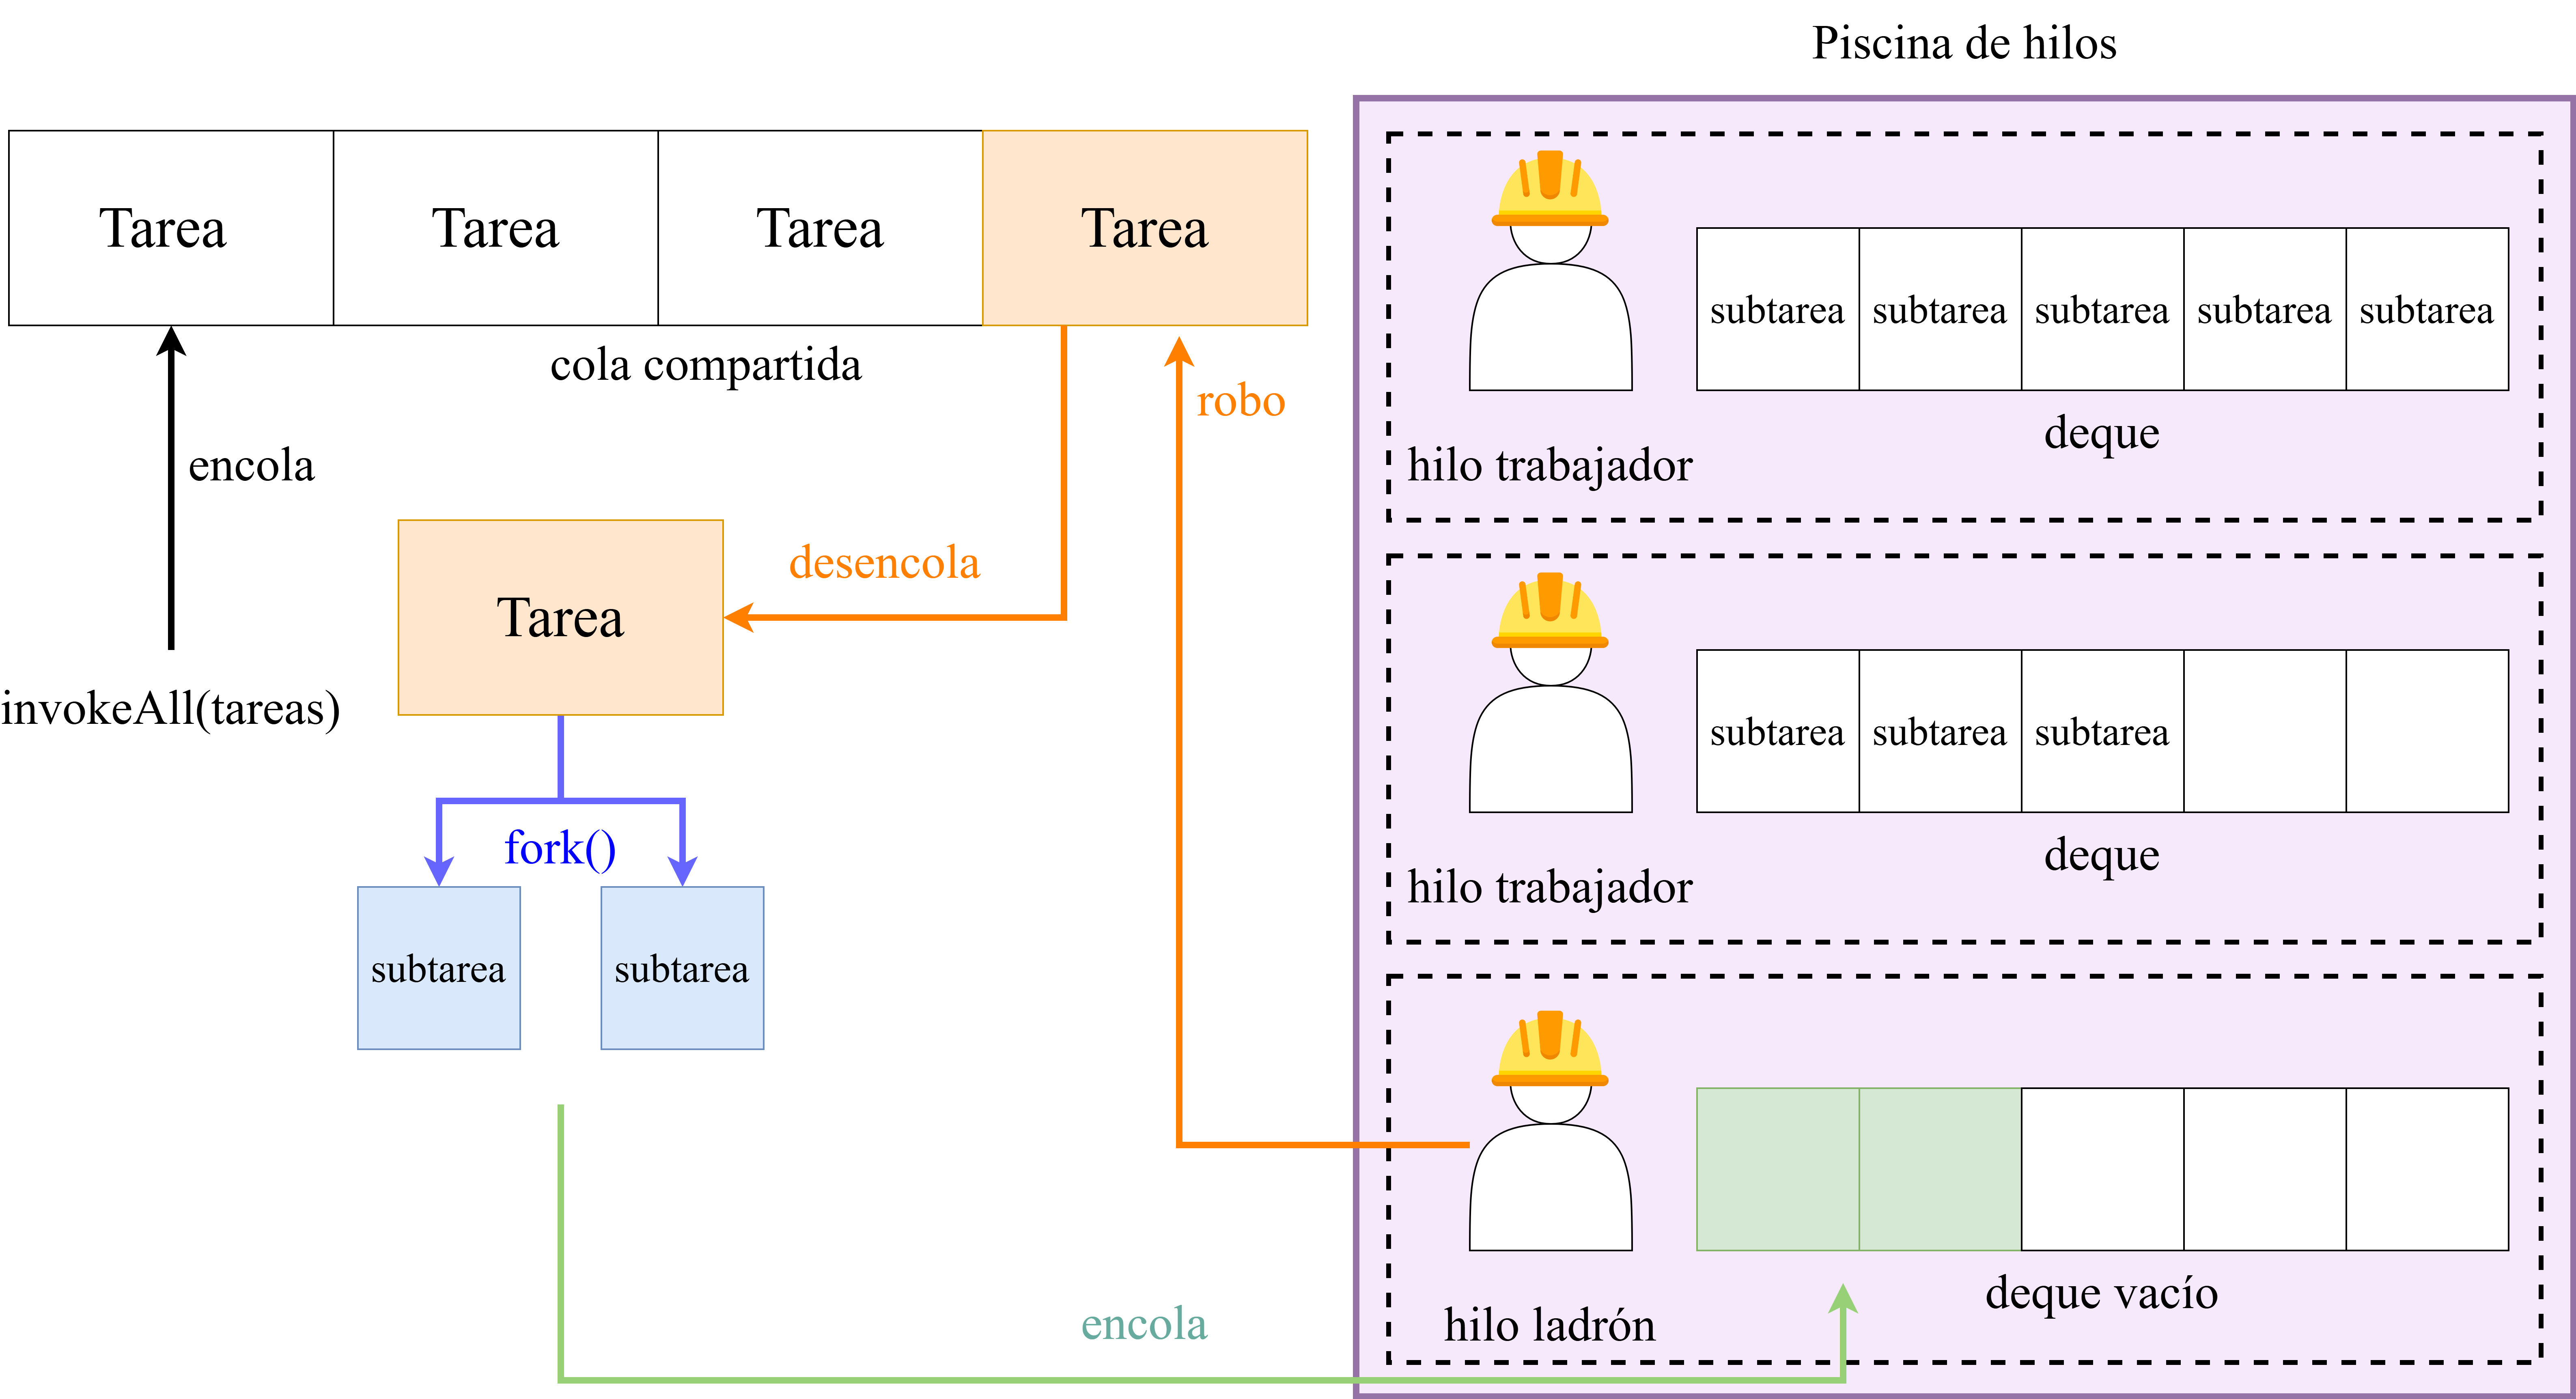
\includegraphics[width=0.85\linewidth]{Diagrames/forkJoinPool.png}
    \caption{Funcionamiento del \lstinline{ForkJoinPool}}
    \label{fig:forkJoinPool}
\end{figure}

Para crear una \lstinline{ForkJoinPool} simplemente se llama a su constructor y se pasa el número de hilos que tendrá la piscina: \lstinline{ForkJoinPool forkjoinpool = new ForkJoinPool(numHilos)}. Existen dos maneras de pasar tareas a una \lstinline{ForkJoinPool}: tareas que no retornan ningún valor (\lstinline{RecursiveAction}) y tareas que sí retornan (\lstinline{RecursiveTask}). Ambas subclases heredan de \lstinline{ForkJoinTask}. \footnote{\cite{OracleForkJoin}}

Concretamente, la lógica del MSRP se inscribe en una clase \lstinline{MergeSortRecursivoParalelo} que hereda de clase abstracta \lstinline{RecursiveAction} como se observa en la Figura \ref{fig:MSRP_RecursiveAction}

\begin{figure}[hbtp]
    \begin{lstlisting}[language=java, frame=single, numbers=left]
    public class MergeSortRecursivoParalelo extends RecursiveAction {
        private final int[] A;
        private final int length;
        private final int threshold = 8192;
        
        public  MergeSortRecursivoParalelo(int[] A, int length){ //Constructor }
        @Override
        protected void compute() { //Logica del Merge Sort }
        public static void merge(int[] A, int[] L, int[] R, int left, int right) {    }
    }
    \end{lstlisting}
    \caption{Esquema de la clase \lstinline{MergeSortRecursivoParalelo}}
    \label{fig:MSRP_RecursiveAction}
\end{figure}

En dicha clase el algoritmo de \textit{Merge Sort} se queda encapsulado en el método abstracto \lstinline{compute()}, como se observa en la Figura \ref{fig:MSRP_Compute}. La primera condición ejecuta el algoritmo iterativo en caso de que la longitud de entrada de la colección sea inferior a un límite. Eso se debe a que llega un momento en que ya no es eficiente generar más subtareas porque el costo de gestión de las subtareas es más elevado que el costo de resolver los subproblemas de forma iterativa. Después se crean dos subtareas, por ahora inactivas, para cada lado de la colección. A continuación, se pasan las subtareas a \lstinline{invokeAll()}, que las encola en la cola compartida de piscina y espera a que \lstinline{Left} y \lstinline{Right} finalicen. Finalmente, se unen las dos partes con el mismo algoritmo \lstinline{merge()} de la implementación recursiva iterativa.

\begin{figure}[hbtp]
    \begin{lstlisting}[language=java, frame=single, numbers=left]
    @Override
    protected void compute() {
        if (length <= threshold) {
            MergeSortRecursivoSerial.sort(A, length);
        } else {
            final int mid = length / 2;
            int[] L = new int[mid];
            int[] R = new int[length - mid];

            for (int i = 0; i < mid; i++)   L[i] = A[i];
            for (int i = mid; i < length; i++)  R[i - mid] = A[i];

            final MergeSortRecursivoParalelo Left = new  MergeSortRecursivoParalelo(L, mid);
            final MergeSortRecursivoParalelo Right = new  MergeSortRecursivoParalelo(R, length - mid);

            invokeAll(Left, Right);

            merge(A, L, R, mid, length - mid);
        }
    }
    \end{lstlisting}
    \caption{Método \lstinline{compute()} del MSRP}
    \label{fig:MSRP_Compute}
\end{figure}

\subsection{Merge Sort Paralelo (MSIP)}
Para la paralelización del algoritmo iterativo se ha hecho uso de la interfaz \lstinline{ExecutorService} que proporciona Java y que proporciona un marco para gestionar y controlar la ejecución de tareas asincrónicas. A diferencia de las piscinas \lstinline{ForkJoin}, el \lstinline{ExecutorService} utiliza un algoritmo de trabajo compartido (\textit{work-sharing algorithm}). Esto implica que solo hay una cola compartida entre todos los hilos: una vez termina un hilo de ejecutar una subtarea, extrae otra de la cola. Este flujo de ejecución es apropiado para tareas independientes entre ellas. 

En este caso, la implementación iterativa paralela se hace en una función \lstinline{sort() } como la de la Figura \ref{fig:MSIP_sort()}. Para crear una instancia de \lstinline{ExecutorService} se usan los métodos que proporciona la clase \lstinline{Executors} de Java. Particularmente, \lstinline{.newFixedThreadPool(numHilos)} crea una piscina con un número de hilos fijo determinado. En este programa se crean un número de hilos correspondiente al número de núcleos disponibles en el ordenador para la JVM. A continuación, para cada iteración se encola en \lstinline{executor} una tarea \lstinline{merge()} mediante una expresión lambda que recibe \lstinline{executor.submit()}. Cada llamada a \lstinline{merge()} es una subtarea más. Estas subtareas se guardan en un objeto de la clase \lstinline{Future} que permite sincronizar la ejecución de tareas, ya que después se llama a \lstinline{future.get()} que obliga al hilo principal a esperar a que acaben todas las tareas encoladas. De lo contrario, podríamos pasar al siguiente \lstinline{size} sin asegurarse de que todas las partes están ordenadas. Una vez completado los bucles se llama a \lstinline{executor.shutdown()}, que espera a que, una vez terminen de ejecutarse todas las tareas encoladas anteriormente, cierra la piscina \lstinline{executor} y libera los hilos.

\begin{figure}
    \centering
    \begin{lstlisting}[language=java, frame=single, numbers=left]
    public static void sort(int[] array) {
        int n = array.length;
        int[] aux = new int[n];
        ExecutorService executor = Executors.newFixedThreadPool(Runtime.getRuntime().availableProcessors());

        for (int size = 1; size < n; size *= 2) {
            for (int left = 0; left < n - size; left += 2 * size) {
                int mid = left + size - 1;
                int right = Math.min(left + 2 * size - 1, n - 1);
                int finalLeft = left; //El resto son efectivamente finales
                Future<?> future = executor.submit(() -> merge(array, aux, finalLeft, mid, right));
                try {
                    future.get(); // Esperar a que la tarea termine
                } catch (Exception e) {
                    e.printStackTrace();
                }
            }
        }
        executor.shutdown();
    }
    \end{lstlisting}
    
    \caption{Método \lstinline{sort()} del MSIP}
    \label{fig:MSIP_sort()}
\end{figure}

\newpage
%%%%%%%%%%%%%%%METODOLOGÍA%%%%%%%%%%%%%%%%%%%%%%
%%%%%%%%%%%%%%%%%%%%%%%%%%%%%%%%%%%%%%%%%%%%%%%%

\section{Parte experimental}

\subsection{Procedimiento}
\begin{enumerate}
    \item Se realizan diez ejecuciones para un \(n\) tamaño de entrada para cada uno de los cuatro algoritmos: MSRS, MSIS, MSRP, MSIP.
    \item Hay 20 \(n\) tamaños que van de 100 hasta 1.000.000.
    \item El tiempo de ejecución se mide mediante la función \lstinline{System.nanoTime} que retorna el tiempo actual más preciso disponible en el sistema. El valor devuelto son los nanosegundos desde un tiempo arbitrario y provee de precisión nanosegundaria, pero no necesariamente exactitud nanosegundaria Cada ejecución se realizan entre una variable \lstinline{long startTime} y \lstinline{long endTime}. El tiempo de ejecución es la diferencia entre estas.\footnote{\cite{OracleSystem}}
    \item Después se elimina el peor y mejor tiempo de entre las diez ejecuciones, quedando así ocho.
    \item Todas las colecciones son generadas mediante la clase \lstinline{SplittableRandom} de Java, que en este caso genera colecciones de tipo \lstinline{int} con valores pseudoaleatorios extraídos de una distribución uniforme. \footnote{\cite{OracleSplittableRandom}}
    \item Antes de cada ejecución se llama al \lstinline{Garbage Collector} asegurar que no haya interferencias de otros procesos.
    \item En el caso de los algoritmos paralelos se establece un mismo número de hilos para cada piscina para que la comparación sea justa.
    \item El código de las implementaciones, el código del \textit{benchmark} y los resultados del \textit{benchmark} quedan recogidos en los Apéndices A, B y C respectivamente.
\end{enumerate}

\subsection{Entorno}
Los algoritmos son ejecutados en un computador con procesador Intel(R) Core(TM) i5-11400F @ 2,60GHz y 16GB de RAM DDR4 3200MHz. En el SO de Windows 10 Pro 22H2 (x64). El IDE de ejecución es IntelliJ Idea Community Edition 2023.3.3.

\section{Discusión de resultados}
\subsection{Comparación}
\subsection{Conclusión}

\section{Bibliografía}
\bibliography{bibliografia}
\section{Anexo}

\end{document}